\documentclass[conference]{IEEEtran}
\IEEEoverridecommandlockouts
% The preceding line is only needed to identify funding in the first footnote. If that is unneeded, please comment it out.
\usepackage{cite}
\usepackage{amsmath,amssymb,amsfonts}
\usepackage{algorithmic}
\usepackage{graphicx}
\usepackage{textcomp}
\usepackage{xcolor}
\usepackage{mathtools}
\usepackage{breqn}
\def\BibTeX{{\rm B\kern-.05em{\sc i\kern-.025em b}\kern-.08em
    T\kern-.1667em\lower.7ex\hbox{E}\kern-.125emX}}
\begin{document}

\title{Safety and stability analysis of FollowerStopper\\
%{\footnotesize \textsuperscript{} }
%\thanks{Identify applicable funding agency here. If none, delete this.}
}

\author{\IEEEauthorblockN{Chris Kreienkamp}
\IEEEauthorblockA{\textit{Department of Aerospace and Mechanical Engineering} \\
\textit{University of Notre Dame}\\
Notre Dame, IN, United States \\
ckreienk@nd.edu}
\and
\IEEEauthorblockN{Daniel Fishbein}
\IEEEauthorblockA{\textit{Physics, Astronomy, and Materials Science Department} \\
\textit{Missouri State University}\\
Springfield, MO, United States \\
fishbein486@live.missouristate.edu}
\and
\IEEEauthorblockN{Rahul Bhadani}
\IEEEauthorblockA{\textit{Department of Electrical and Computer Engineering} \\
\textit{University of Arizona}\\
Tucson, AZ, United States \\
rahulbhadani@email.arizona.edu}
\and
\IEEEauthorblockN{Jonathan Sprinkle}
\IEEEauthorblockA{\textit{Department of Electrical and Computer Engineering} \\
\textit{University of Arizona}\\
Tucson, AZ, United States \\
sprinkjm@email.arizona.edu}
}

\maketitle

\begin{abstract}
In this paper we demonstrate that the velocity controller, FollowerStopper, is safe and string unstable. FollowerStopper is a controller that is meant to be implemented on an autonomous vehicle or in an adaptive cruise control (ACC) system. Through mathematical proof, simulation in Simulink, and hardware in the loop implementation on a real autonomous vehicle through Robot Operating System (ROS) and Gazebo, several results are achieved. It is found that an autonomous vehicle controlled by FollowerStopper will never crash. FollowerStopper will dissipate larger traffic waves from human-driven vehicles but will amplify smaller velocity perturbations that are created within the controller. Given the maximum LiDAR range of 81 m, FollowerStopper will never command a velocity greater than 13.69 m/s.
\end{abstract}



%%%%%%%%%%%%%%%%%%%%%%%%%%%%%%%%%%%%%%%%%%%%%%%%%%%%%%%
%%%%%%%%%%%%%%%%%%%%%%%%%%%%%%%%%%%%%%%%%%%%%%%%%%%%%%%
%%%%%%%%%%%%%%%%%%%%%%%%%%%%%%%%%%%%%%%%%%%%%%%%%%%%%%%



%\begin{IEEEkeywords}
%component, formatting, style, styling, insert
%\end{IEEEkeywords}


%%%%%%%%%%%%%%%%%%%%%%%%%%%%%%%%%%%%%%%%%%%%%%%%%%%%%%%
%%%%%%%%%%%%%%%%%%%%%%%%%%%%%%%%%%%%%%%%%%%%%%%%%%%%%%%
%%%%%%%%%%%%%%%%%%%%%%%%%%%%%%%%%%%%%%%%%%%%%%%%%%%%%%%


\section{Introduction and Related Work}
In order to maintain safety while driving, humans need a certain amount of safe distance between their car and the car directly in front of them so that if the car in front stops abruptly, they can react and stop in time to prevent a crash. From here forward the car which is of interest will be termed the autonomous vehicle (AV) and the car directly in front will be termed the lead vehicle. If the cars are traveling at a slow speed, the AV can follow at a closer distance because the car will not travel as far during the time it takes to react to the lead and to brake.
When the number of cars on a section of highway increases, the car density increases, often termed as congestion. When highways are congested, cars must travel closer together than they normally would, so drivers must drive slower than the speed limit to maintain safety.

It was shown that humans, once the congestion reaches a certain threshold, will inevitably cause traffic jams. This will occur even if there are no traffic triggers, termed bottlenecks, such as lane changes, merges, tunnels, or other physical hindrances \cite{sugiyama2008traffic}. The reason for the formation of these "phantom traffic jams" is that humans are only concerned with maintaining safety, but are typically not concerned about dissipating traffic. When a driver brakes, for example, the driver behind will often brake harder, and this chain of events will continue until cars must come to a complete stop. It is even proposed that bottlenecks lead to traffic jams because such events will cause the car density to exceed the threshold \cite{sugiyama2008traffic}.

Throughput is the number of cars that pass through a given area over a certain time. The best alternative to traffic jams, meaning the situation which will allow for the greatest throughput, is for all of the cars to follow the same optimal velocity. In doing so, there will be no hard braking or quick acceleration, further providing benefits of improved fuel economy, less wear on the brake pads and engine, and preventing the frustration and stress that accompanies road rage. The throughput is highest when setting the optimal velocity of the autonomous vehicle to be the average speed of the traffic wave ahead \cite{stern2018dissipation}.

With the development of new ACC and autonomous systems, a larger percentage of cars on the road will have some degree of automation. It will take many decades for all cars on the road to be autonomous, so it is critical to inspect the impact that just a few autonomous vehicles will have on the overall traffic flow. Stern et al. demonstrated that even a small percentage of autonomous vehicles ($<5\%$) could have a substantial effect in reducing traffic \cite{stern2018dissipation}. Some researchers suspect that between 2020 and 2040 there could be the development of highway lanes solely for autonomous vehicles \cite{litman2017autonomous}, at which point designers could rely on vehicle-to-vehicle communication with the formation of high-density platoons. Until then, however, it is necessary to design autonomous vehicles and ACC systems with the ability to safely interact with imperfect and unpredictable human drivers. To optimize the situation, the autonomous systems should be safer than human drivers and should do as much as they can to reduce traffic.

One such velocity controller is FollowerStopper, developed and tested in a variety of papers and experiments predominantly by the University of Arizona CAT Vehicle team \cite{stern2018dissipation, bhadani2019real, bhadani2018dissipation}. \cite{bhadani2018dissipation} merely demonstrates that FollowerStopper can avoid collision and dampen traffic waves, but it does not assure safety or prove string stability.


%%%%%%%%%%%%%%%%%%%%%%%%%%%%%%%%%%%%%%%%%%%%%%%%%%%%%%%
%%%%%%%%%%%%%%%%%%%%%%%%%%%%%%%%%%%%%%%%%%%%%%%%%%%%%%%
%%%%%%%%%%%%%%%%%%%%%%%%%%%%%%%%%%%%%%%%%%%%%%%%%%%%%%%



\section{Setup}
Suppose there is a line of vehicles in a straight infinite lane that never has any lane changes or other bottlenecks, as pictured in Figure \ref{fig1}. In Figure \ref{fig1}, the middle car is vehicle $i$. The vehicle to the right is vehicle $i-1$, and the trend continues so that the vehicle at the very front of the line of vehicles will be vehicle 1. The vehicle to the left is vehicle $i+1$, and the trend continues so that the vehicle at the very end of the line of $n$ vehicles will be vehicle $n$. The x-position of 0 is an arbitrary location, but for ease it can be thought of as the starting position of the last vehicle in the line such that at all times $t\geq 0$, the position of every vehicle $x_i\geq 0$.

\begin{figure}[htbp]
\centerline{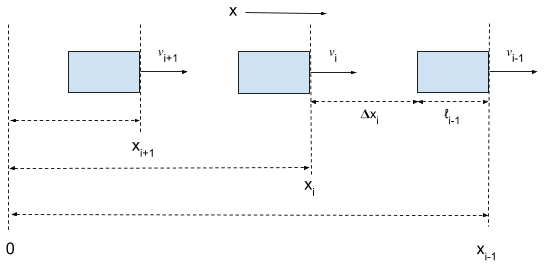
\includegraphics[width=3.75 in]{carLane.png}}
\caption{Line of vehicles in a straight lane.}
\label{fig1}
\end{figure}

\subsection{Variables}
\subsubsection{Relative distance, $\Delta x_i$} 
The relative distance for vehicle $i$ is the distance between the front bumper of vehicle $i$ and the back bumper of vehicle $i-1$. That is,
\begin{eqnarray}
\Delta x_i = x_{i-1}-x_i-l_{i-1},
\end{eqnarray}
where $x_{i-1}$ is the position of the front bumper of vehicle $i-1$, $x_i$ is the position of the front bumper of vehicle $i$, and $l_{i-1}$ is the length of vehicle $i-1$.
\subsubsection{Relative velocity, $\Delta v_i$}
The relative velocity for vehicle $i$ is the velocity difference between vehicle $i-1$ and vehicle $i$. That is,
\begin{eqnarray}
\Delta v_i=v_{i-1}-v_i,
\end{eqnarray}
where $v_{i-1}$ is the velocity of vehicle $i-1$ and $v_i$ is the velocity of vehicle $i$.
\subsubsection{Reference velocity, $r$}
Also known as the desired velocity or optimal velocity, the reference velocity is the velocity at which the autonomous vehicle desires to travel. It is typically the average velocity over the length of a traffic wave, and is found by dividing the total distance traveled by a vehicle in front of the AV by the time. That is,
\begin{eqnarray}
r={d_{total}\over t_{total}}
\end{eqnarray}
The reference velocity is typically sent to the AV by means of a roadside controller.
\subsubsection{Spacing error, $\epsilon_i$}
The spacing error is the difference between the desired relative distance and the actual relative distance, giving,
\begin{eqnarray}
\epsilon_i = \Delta x_{i des}-\Delta x_i.
\end{eqnarray}

\subsection{Definitions}
\subsubsection{Safe}
A scenario is safe if at all times for every vehicle $i$ such that $1<i\leq n$, then $\Delta x_i>0$ m. This means that the relative distance will always be greater than 0 for every vehicle.
\subsubsection{Individual vehicle stable}
A velocity control law is considered to be individual vehicle stable if the spacing error of the AV approaches 0 with time if the lead vehicle travels at a constant velocity.
\subsubsection{String stable}
When a lead vehicle accelerates or decelerates in front of an individual vehicle stable AV, the spacing error will momentarily be nonzero. Suppose there is an infinite line of autonomous vehicles with one lead vehicle in front. The velocity control law is considered to be string stable if, during acceleration or deceleration of the lead vehicle, the spacing error decreases with each successive vehicle as they react to the change in velocity \cite{rajamani2011vehicle}. Additionally, all spacing errors must be in the same direction, either all negative or all positive for a particular change in velocity. \cite{feng2019string} displays a theoretical plot of the spacing error of a string unstable and string stable group of vehicles, reproduced in Figure \ref{stringexample}.

\begin{figure}[htbp]
\centerline{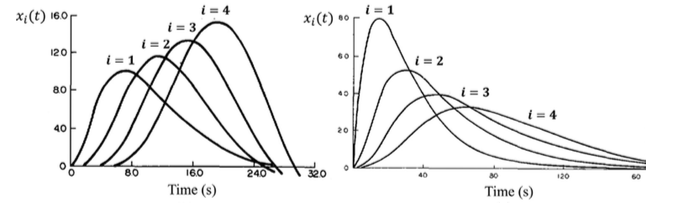
\includegraphics[width=3 in]{stringexample}}
\caption{String unstable and string stable spacing error vs time representation.}
\label{stringexample}
\end{figure}

\subsection{Infrastructure}
The FollowerStopper velocity controller is first modeled in Simulink and then used in conjunction with ROS to test in the physics-based simulation engine, Gazebo. After demonstrating success in Gazebo, the velocity controller is implemented onto the Cognitive and Autonomous Test (CAT) Vehicle at the University of Arizona using a hardware in the loop (HIL) configuration as described in \cite{bhadani2018cat}.

\hspace{0.01 in}The CAT Vehicle is a modified Ford Hybrid Escape with a SICK LMS 291 Front Laser Rangefinder, a Velodyne HDL-64E S2 LiDAR, two Pointgrey Firefly MV FFMV-03M2C cameras, and a Novatel VPS/IMU. The FollowerStopper velocity controller uses distance data from the LiDAR to determine the relative distance to the car in front $\Delta x_i$. Using the relative distance data, the AV can determine the relative velocity \cite{bhadani2019real}. Assuming that the AV knows its own velocity at all times, it can use the relative velocity data to determine the velocity of the lead vehicle.



%%%%%%%%%%%%%%%%%%%%%%%%%%%%%%%%%%%%%%%%%%%%%%%%%%%%%%%
%%%%%%%%%%%%%%%%%%%%%%%%%%%%%%%%%%%%%%%%%%%%%%%%%%%%%%%
%%%%%%%%%%%%%%%%%%%%%%%%%%%%%%%%%%%%%%%%%%%%%%%%%%%%%%%



\section{Parameters}
In the development of the FollowerStopper controller, several parameters are often used. They are grouped here to allow for easy reference. Some of the parameters involve acceleration due to gravity, which will be taken as $G=9.80665 {m\over s^2}$ for our purposes. In choosing the parameters, safety is the priority. If safety is not a concern, keeping a small distance between the AV and the lead is desirable in order to accommodate for a higher density of cars on the road and to prevent lane changes of human drivers in front of the AV. Table \ref{tab1} at the end of the section summarizes the findings.
 
\subsection{Minimum relative distance, $\psi$}
Minimum relative distance refers to the minimum acceptable distance between the AV and the lead. While stopped, it is expected that $\Delta x= \psi$. We chose an arbitrary value of $\psi=1$ because we thought that if the AV was any closer to the lead, the passengers of the AV might be uncomfortable because they do not have control of the car. 

\subsection{Comfortable acceleration, $a_{cmft}$}
The comfortable acceleration limits the maximum acceleration of the AV. When the reference velocity increases, the AV will not immediately travel at the reference velocity, but will increase its velocity at an acceleration of $a_{cmft}$. Particularly in congested traffic conditions, it is undesirable for the AV to have jerky velocity changes. Though it is essential to safety to leave the deceleration of the AV unrestrained, limiting the acceleration will provide for greater passenger comfort and expectability. {comfortable acceleration} details comfortable accelerations in the range of $0.11G$ to $0.15G$ for public mass transportation systems. Because passengers will be much less affected by a car's acceleration due to comfortable seating and expectability than a public mass transport acceleration, we chose $0.15G$ a reasonable value.

\subsection{Comfortable deceleration, $a_{dcmft}$}
The comfortable deceleration defines the maximum amount by which the reference velocity can change. In cases where the reference velocity drops to a much lower value, it is not required for the AV to immediately travel at that value in order to remain safe. $a_{dcmft}$ ensures a smooth transition when safety is not of concern. \cite{hoberock1977survey} details $0.266G$ as a deceleration that is comfortable to passengers and is preferred by a driver.

\subsection{Maximum acceleration, $a_{max}$}
The maximum acceleration refers to the maximum possible acceleration of the AV. Fiver different websites \cite{carsort,motortrend,caranddriver,edmunds,michigan} listed different maximum acceleration data for the Ford Escape Hybrid, which is the vehicle under consideration. The data was based off an experiment where the vehicle would start at a stop and would accelerate as quickly as possible to 60 mph. For safety purposes, the largest acceleration was chosen as the maximum acceleration for the Ford Escape Hybrid, that is $3.53 {m\over s^2}$ \cite{motortrend}. If the maximum acceleration of the AV is not known, \cite{hoberock1977survey} details $3.34 {m\over s^2}$ as a reasonable maximum acceleration. This can be used if a more accurate estimation cannot be found.

\subsection{Maximum deceleration, $a_{dmax}$}
The maximum deceleration refers to the maximum possible deceleration of the AV. Five different websites \cite{carsort,motortrend,caranddriver,edmunds,michigan} listed different maximum deceleration data for the Ford Escape Hybrid. The data was based off of an experiment where the vehicle would travel at a constant velocity before braking as hard as possible, and then reporting the stopping distance. For safety purposes, the deceleration with the lowest absolute value was chosen as the maximum deceleration for the Ford Escape Hybrid, that is $-7.66{m\over s^2}$ \cite{caranddriver}. If the maximum deceleration of the AV is not known, \cite{fambro1997nchrp} details $-3.99{m\over s^2}$ as the maximum deceleration of a passenger car traveling on wet pavement. This can be used if a more accurate estimation cannot be found.

\subsection{Deceleration ratio, $k$}
The deceleration ratio is the ratio between the maximum deceleration of the lead vehicle and the maximum deceleration of the AV. For FollowerStopper to be safe, as is shown in the next section, there must be some knowledge of how the lead and AV accelerations relate. A deceleration ratio less than unity, that is $k<1$, means that the AV can decelerate to a stop faster than the lead, meaning that it can travel closer than normal to the lead and still be safe. A deceleration ratio greater than unity, that is $k>1$, means that the lead can decelerate to a stop faster than the AV, meaning that the AV must follow at a greater relative distance in order to have a greater stopping distance. To be safe, assume that the lead vehicle can decelerate as fast as physically possible. From section A of the Appendix, the deceleration of a vehicle is $a=-G\mu$, where $\mu$ is the coefficient of friction. \cite{muller2003estimation} concludes that the maximum tire-road friction coefficient in normal driving on a dry road is $\mu_{max}=1$, so the maximum deceleration of the lead vehicle is $-G$.

\begin{table}[htbp]
\caption{FollowerStopper Parameters}
\begin{center}
\begin{tabular}{|c|c|c|c|}
\hline
\textbf{Name} & \textbf{Symbol} & \textbf{Calculation} & \textbf{Value} \\
\hline
					&				&						&					\\
minimum relative distance	&	$\psi$		&	---					&	1				\\
					&				&						&					\\
comfortable acceleration	&	$a_{cmft}$	&	$0.15\cdot G$			&	1.47$m\over s^2$	\\
					&				&						&					\\
comfortable deceleration	&	$a_{dcmft}$	&	$-0.266\cdot G$		&	-2.61$m\over s^2$	\\
					&				&						&					\\
maximum acceleration	&	$a_{max}$	&	---					&	3.53$m\over s^2$	\\
(Ford Escape Hybrid)	&				&						&					\\
maximum deceleration	&	$a_{dmax}$	&	---					&	-7.66$m\over s^2$	\\
(Ford Escape Hybrid)	&				&						&					\\
deceleration ratio		&	$k$			&	$-G\over a_{dmax}$		&	1.28				\\
(Ford Escape Hybrid)	&				&						&					\\

\hline
\end{tabular}
\label{tab1}
\end{center}
\end{table}



%%%%%%%%%%%%%%%%%%%%%%%%%%%%%%%%%%%%%%%%%%%%%%%%%%%%%%%
%%%%%%%%%%%%%%%%%%%%%%%%%%%%%%%%%%%%%%%%%%%%%%%%%%%%%%%
%%%%%%%%%%%%%%%%%%%%%%%%%%%%%%%%%%%%%%%%%%%%%%%%%%%%%%%



\section{FollowerStopper Description}

\subsection{Classification}
The premise of FollowerStopper is to command exactly the reference velocity $r$ whenever safe because this is the velocity that could dissipate already formed traffic jams and could prevent new traffic jams from forming. Assuming that the lead starts a safe distance ahead of the AV, when $r\leq v_{lead}$, FollowerStopper will command the reference velocity, that is $v_{cmd}=r$. FollowerStopper takes the AV's velocity, relative velocity to the lead vehicle, and relative distance to the lead vehicle as inputs to determine three relative distances $\xi_1$, $\xi_2$, and $\xi_3$, in order of increasing magnitude.

Suppose now that $r>v_{lead}$, so the relative distance $\Delta x$ will be decreasing. Once the AV gets within the relative distance $\Delta x \leq \xi_3$,  FollowerStopper will slow down the vehicle by commanding a velocity less than $r$. If the AV must continue to travel at a value lower than the relative velocity $r$, FollowerStopper, by slowly decreasing the command velocity, will cause the AV to travel at the lead velocity $v_{lead}$, following at a relative distance of $\Delta x=\xi_2$. If the lead vehicle decelerates unexpectedly or the relative distance decreases further to $\Delta x=\xi_1$, FollowerStopper will command the AV to stop.

The mathematical representation of the FollowerStopper controller from \cite{bhadani2019real} is reproduced below. 
\begin{eqnarray}
v_{cmd} &=& \begin{dcases}
        0 								& \Delta x\leq \xi_1 \\
        v{\Delta x-\xi_1\over\xi_2-\xi_1} 			& \xi_1< \Delta x\leq \xi_2 \\
        v+(r-v){\Delta x-\xi_2\over\xi_3-\xi_2}			& \xi_2< \Delta x\leq \xi_3 \\
        r 								& \xi_3< \Delta x \\
    \end{dcases}
\end{eqnarray}
\begin{eqnarray}
\xi_j(\Delta v)	&=& \omega_j + {1\over 2\alpha_j}(\Delta v^*)^2 \ \ {\rm for \ \ j=1, 2, 3}
\end{eqnarray}
where $v = min(max(v_{lead}, 0), r)$. $r$ is the reference velocity as taken from the output of smoothUpParams and $v_{cmd}$ is the command velocity that is sent to the AV. The $\omega_j$ and $\alpha_j$ values in the equation for $\xi_j$ are distance and deceleration parameters, respectively, and $\Delta v^*=min(\Delta v, 0)$. \cite{bhadani2019real} suggests for future work to optimize the distance and deceleration parameters, which were previously set to $\omega_1=4.5$ m, $\omega_2=5.25$ m, $\omega_3=6.0$ m, $\alpha_1=1.5 {\rm {m\over s^2}}$, $\alpha_2=1.0 {\rm {m\over s^2}}$, and $\alpha_3=0.5 {\rm {m\over s^2}}$. The following sections seek to accomplish this task of finding the ideal $\xi_j$ values.

\subsection{SmoothUpParams}
Theoretically, the reference velocity will be given to the AV by means of a roadside controller which takes traffic data and determines the optimal constant velocity. SmoothUpParams is a function of the new reference velocity $r$, the autonomous vehicle velocity $v_{AV}$, the maximum comfortable acceleration of the autonomous vehicle $a_{cmft}$, and the maximum comfortable deceleration of the autonomous vehicle $a_{dcmft}$. Using these inputs, SmoothUpParams edits the reference velocity so that it is a reasonable value when it is sent to the FollowerStopper controller. Suppose, for example, the speed limit and consequently the reference velocity were to change from 10 m/s to 15 m/s and no car was in front of the AV. Without SmoothUpParams, FollowerStopper would command the AV to travel at the reference velocity of 15 m/s immediately, but this will result in an unnecessarily large acceleration. SmoothUpParams will cause the reference velocity to increase at a slow rate so that FollowerStopper can comfortably transition to the new reference velocity without accelerating faster than $a_{cmft}$ or decelerating faster than $a_{dcmft}$.

\subsection{Designing $\xi_1$ for safety}
According to FollowerStopper, if $\Delta x \leq \xi_1$, then $v_{cmd}=0$. That is, if the relative distance between the AV and the lead is less than or equal to $\xi_1$, the AV should brake as hard as possible or remain stopped if already at a stop. If FollowerStopper commands $v_{cmd}=0$, the AV will not initiate the emergency braking command until $\delta$ seconds after the FollowerStopper command due to system delay. To prove that FollowerStopper is safe, it must be shown that if $\Delta x = \xi_1$, braking as hard as possible after a delay of $\delta$ seconds will never result in a crash. This assumes that no unexpected obstacle comes between the AV and the lead. The metric is computed as:
\begin{dmath}
\xi_1 = \psi +\Delta v^{**}+v_{AV}(1-{a_{max}\over a_{dmax}})\delta+{a_{max}\over 2}(1-{a_{max}\over a_{dmax}})\delta^2
\end{dmath}
where $\Delta v^{**} = max(0,{1\over 2ka_{dmax}}(v_{lead}^2-kv_{AV}^2))$. The derivation can be found in section B the Appendix.

\subsection{Designing $\xi_2$ for string stability}
When $v_{AV}>v_{lead}$, the relative distance $\Delta x$ will decrease as the AV approaches the lead. When $\Delta x$ drops below $\xi_3$, FollowerStopper is designed to incrementally command a smaller velocity until the command velocity is equal to the velocity of the lead $v_{cmd}=v_{lead}$. Once $v_{AV}=v_{lead}$, the AV will maintain the distance $\Delta x=\xi_2$. If the relative distance drops below this equilibrium distance, that is $\Delta x<\xi_2$, the velocity of the AV will decrease below $v_{lead}$ in an attempt to recover this distance.

 If the distance is greater than the equilibrium distance, that is $\Delta x>\xi_2$, the velocity of the AV will increase in an attempt to recover this distance unless $v_{lead}$ exceeds the reference velocity, at which point $v_{cmd}=r$. Therefore, the AV will spend the majority of its functioning at or above the distance $\xi_2$. It is important, then, that $\xi_2$ is a string stable distance. According to \cite{rajamani2011vehicle}, string stability is maintained when the time-gap $h$ between two cars is such that $h\geq2\tau$, where $\tau$ is the time constant of any lags in tracking the command velocity, or in other words, it is the delay of the system $\delta$. It is reasonable to treat the relative distance $\xi_1$ as the point from which to maintain a time-gap greater than $2\delta$ because at $\Delta x=\xi_1$, the AV must stop. With this knowledge the metric is computed as: 
 \begin{dmath}
 \xi_2 = \xi_1 + 2v_{AV}\delta
 \end{dmath}

\subsection{Designing $\xi_3$ for comfort}
If $\Delta x>\xi_3$, then $v_{cmd}=r$. When $\Delta x\leq \xi_3$, the AV will begin a comfortable deceleration from $r$ to $v_{lead}$, maintaining the distance $\xi_2$ while it travels at $v_{lead}$. In order to preserve an equal spacing between all of the relative distance parameters $\xi_3$, $\xi_2$, and $\xi_1$, FollowerStopper is designed such that $\xi_2$ is the average of $\xi_1$ and $\xi_3$. A brief amount of algebra reveals the calculation for $\xi_3$. The metric is computed as:
\begin{eqnarray}
\xi_3 = 2\xi_2-\xi_1
\end{eqnarray}

\subsection{Maximum FollowerStopper speed}
Due to the limited sight of the LiDAR, the AV can only detect relative distance data up to 81 m ahead. Therefore, if there is no obstacle within 81 m, FollowerStopper will assume that there is a vehicle at $\Delta x=81$ m traveling at the same speed as the AV. In such a case, the AV will continue to accelerate until $\xi_2=81$ m because at this point, the AV will no longer accelerate or decelerate unless the lead changes its velocity, which will never happen. $\xi_2=81$ m when $v_{AV}=13.69$ m/s, so the current implementation of FollowerStopper makes it impossible for the AV to travel faster than that speed. The maximum speed would increase if either there was a new formula for $\xi_2$ that would make it smaller, or if the range of the sensors were to increase, for example with the use of radar instead of LiDAR. In our testing we only incorporated LiDAR, however, so we used 81 m as the maximum distance of a vehicle ahead.

\subsection{Further considerations}
FollowerStopper is designed such that the AV will not accelerate faster than $a_{max}$ and will not decelerate faster than $a_{dmax}$. This is necessary because even if FollowerStopper commands an acceleration outside of this range, it is physically impossible for the AV to execute the command. If FollowerStopper were to command an unrealistic velocity, it could cause irreparable wear on the tires or and excessive load to the engine. Additionally, in order to reduce oscillatory noise in the command velocity data, the FollowerStopper controller, after determining a new command velocity, will take a moving average of the new value and a set number of previous $v_{cmd}$ values. The current controller uses a moving average of 75 steps, meaning that the command velocity will be the average of the newly calculated $v_{cmd}$ and the 74 previous command velocities. The reason for this choice is detailed in the section 6.



%%%%%%%%%%%%%%%%%%%%%%%%%%%%%%%%%%%%%%%%%%%%%%%%%%%%%%%
%%%%%%%%%%%%%%%%%%%%%%%%%%%%%%%%%%%%%%%%%%%%%%%%%%%%%%%
%%%%%%%%%%%%%%%%%%%%%%%%%%%%%%%%%%%%%%%%%%%%%%%%%%%%%%%



\section{Simulink Model}
To compare the old and new versions of FollowerStopper, a Simulink model was developed incorporating the Vehicle Body 3DOF model. The model incorporates expected sensor and actuation delays and can display output such as the lead and AV velocities, positions, and accelerations. It is not completely accurate, as when sending a delayed $v_{AV}$ to the Vehicle Body 3DOF block, the simulation produces inaccurate data. Therefore, the $v_{AV}$ data could not be delayed. The final representation of the model is displayed below for a lead vehicle and AV. The model is computed using a fixed time-step of 0.01 s, meaning that it is updated every 0.01 s.

\begin{figure}[htbp]
\centerline{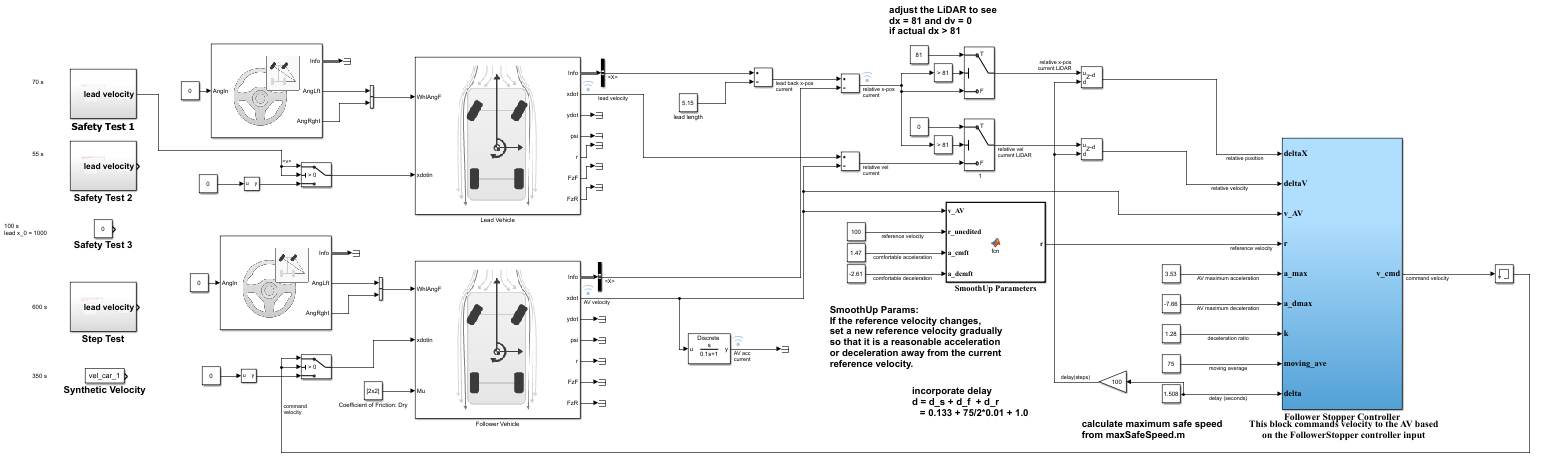
\includegraphics[width=3.5 in]{simulink_model.PNG}}
\caption{Simulink model.}
\label{fig2}
\end{figure}

\subsection{Vehicle Body 3DOF}
The Vehicle Body 3DOF Dual Track block in Simulink models the lead vehicle and the AV. This particular block is ideal for creating virtual sensor data, which can then be used by FollowerStopper. Further information about the model can be found in \cite{vehicledynamicsblockset}. By inputing a velocity "xdot", steering angle, and initial longitudinal position "X\_o" to the lead vehicle, the block artificially creates vehicle data including the instantaneous position and instantaneous velocity of the lead. Another Vehicle Body 3DOF Dual Track block models the AV, using the same steering angle, but starting behind the lead at a lesser longitudinal position "X\_o". The input velocity for the AV comes from the command velocity $v_{cmd}$ output of FollowerStopper.

\begin{figure}[htbp]
\centerline{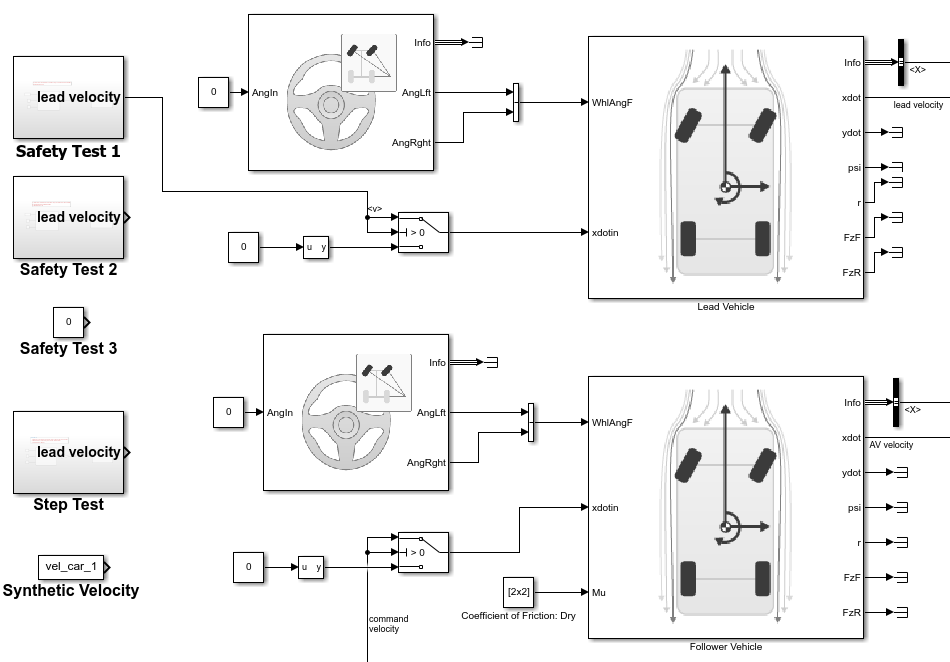
\includegraphics[width=3.5 in]{vehicle_body_3dof.PNG}}
\caption{Lead vehicle and AV model in Simulink using the Vehicle Body 3DOF Dual Track block.}
\label{fig2}
\end{figure}

Several velocity data files were created for the lead to follow to test the safety, string stability, and overall response of the AV to different velocities and accelerations. One particular velocity data file used the exact velocity of a human-driven car from \cite{wu2018arizona}. In Experiment E, car 1 was chosen as the vehicle off of which to obtain a synthetic lead vehicle velocity because Experiment E features the most oscillatory traffic without intervention by the CAT Vehicle to modify the flow of cars. Information about the other experiments in the dataset can be found in \cite{wu2019tracking}.


\subsection{Delay}
The delay $\delta$ of the system is of supreme importance because at high speeds, the AV can travel a considerable distance before receiving and implementing a new velocity command. Contributions to the delay include the LiDAR sensor delay (0.133 s), the moving average filter delay ($\rm {75\ moving\ steps\over 2}(0.01{s\over step})$), and a fixed delay (1.0 s) due to friction, actuator dynamics, controller update rate, etc. From \cite{bhadani2019real}, considering that the position sampling frequency $F_s$ and velocity sampling frequency $F_v$ are both 75 Hz,

\begin{eqnarray*}
\delta &=& {\delta_f F_s \over F_v}+\delta_r = \delta_f +\delta_r \\
&=& 0.133+{75\over 2}(0.01)+1\\
&=& 1.508 \rm\ s
\end{eqnarray*}

where $\delta_f$ is the filter delay and $\delta_r$ is the fixed delay. It is desirable to replicate the actual CAT Vehicle in the Simulink model as nearly as possible. As mentioned above, the LiDAR takes relative distance data, which needs to be filtered to become relative velocity data, adding the 0.133 s sensor delay. Assuming that the AV velocity is known at all times, the AV velocity, relative distance, and relative velocity go as inputs into FollowerStopper. The command velocity $v_{cmd}$ is modified with a moving average filter, adding the 0.375 s filter delay. Once there is a $v_{cmd}$ value, it is sent to the actuators, adding the 1.0 s delay. 

It is obvious that it would be inaccurate to use the current values of the relative distance, relative velocity, and AV velocity in the Simulink model. Though the AV knows its velocity at the time the LiDAR data is processed, it should use the velocity from 0.133 s beforehand, when it received the LiDAR data. It is currently unclear as to which value of the AV velocity FollowerStopper uses in the CAT Vehicle. 

Given this knowledge, the Simulink model could be considered reasonably accurate if the relative distance, relative velocity, and AV velocity were all delayed by 1.508 s. Unfortunately, when the AV velocity is delayed, the simulation updates $v_{cmd}$ once every 1.508 s, slowing the simulation from its normal update rate of 0.01 s. The problem is related to the Vehicle Body block rather than FollowerStopper, and a solution could not be found that would not compromise more important parts of the model. The model therefore uses the delayed relative distance and relative velocity values, but it uses the current AV velocity, deeming the model inaccurate but still an acceptable platform from which to test FollowerStopper before implementation into Gazebo or the actual CAT Vehicle.

\begin{figure}[htbp]
\centerline{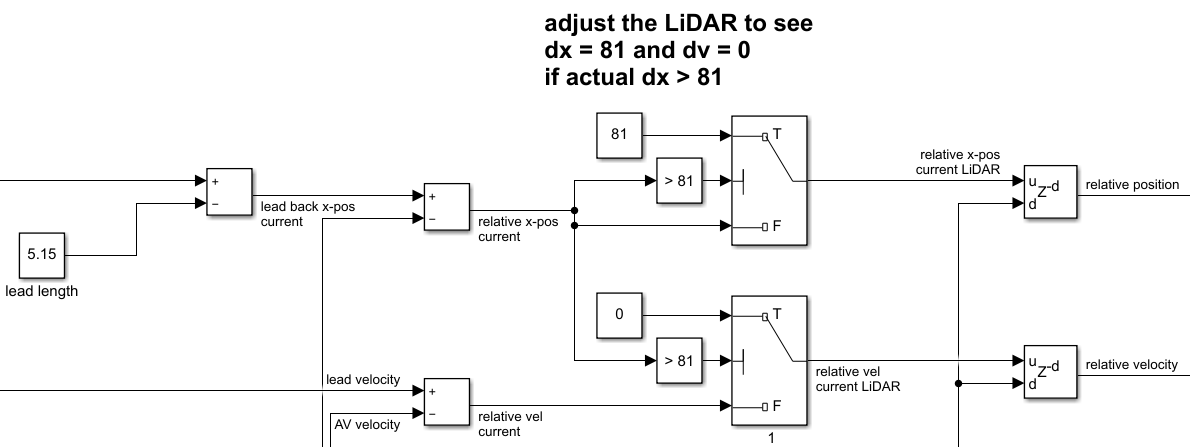
\includegraphics[width=3.5 in]{delay.PNG}}
\caption{Delay in Simulink.}
\label{fig2}
\end{figure}

\subsection{SmoothUpParams}
The SmoothUpParams block, as described above, edits the reference velocity before sending it to FollowerStopper. If the reference velocity changes, most likely due to a road-side controller sending information to the AV, SmoothUpParams will slowly and continually update the reference velocity sent to FollowerStopper. SmoothUpParams will ensure that, if FollowerStopper is commanding exactly the reference velocity, the changing reference velocity will not cause the AV to exceed a maximum comfortable acceleration or deceleration. Once SmoothUpParams reaches the actual reference velocity, it will simply continue to send the current reference velocity until it receives a new one. Our tests never include a changing reference velocity, so SmoothUpParams could technically be removed from the model and nothing would change. However, if further work were to be done in optimizing the reference velocity, SmoothUpParams would be essential.

\begin{figure}[htbp]
\centerline{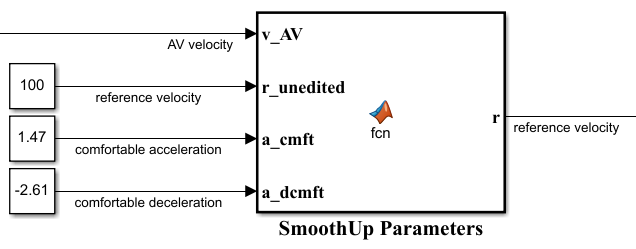
\includegraphics[width=3.5 in]{smoothupparams.PNG}}
\caption{SmoothUpParams in Simulink.}
\label{fig2}
\end{figure}

\subsection{FollowerStopper}
The FollowerStopper block takes $\Delta x$, $\Delta v$, $r$, $a_{max}$, $a_{dmax}$, $k$, the moving average, and $\delta$ as inputs and uses a MATLAB Function to calculate $\xi_1$, $\xi_2$, $\xi_3$, and $v_{cmd}$ as described in section 4 above. The FollowerStopper block outputs the new $v_{cmd}$, and then that value is used as the input velocity to the AV for the next time step.

\begin{figure}[htbp]
\centerline{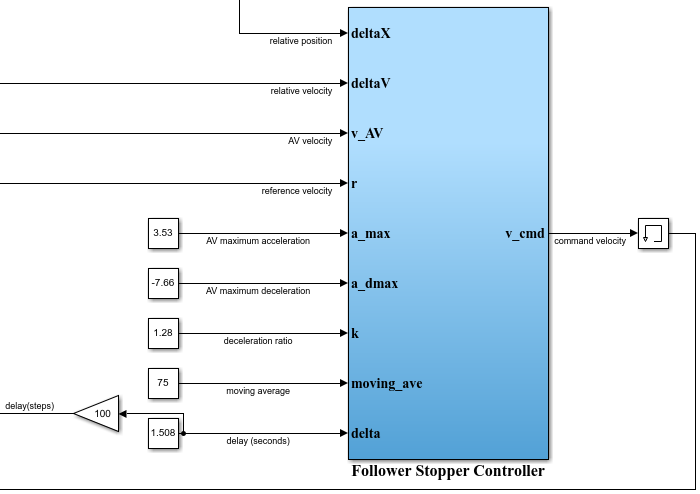
\includegraphics[width=3.5 in]{followerstopper.PNG}}
\caption{FollowerStopper in Simulink.}
\label{fig2}
\end{figure}

\subsection{Multi-car model}
The descriptions thus far have focused on the development of a two-car model, with one lead vehicle and one AV. This is sufficient for building the model, implementing in Gazebo, and testing with the CAT Vehicle. Additionally it is sufficient for determining if FollowerStopper is safe because any velocity can be input to the lead, and the AV will follow. When determining string stability, however, a multi-car model is required in order to see how each successive car reacts to a change in velocity by the lead vehicle. To test for string stability, the AV Vehicle Body 3DOF block, delay blocks, SmoothUpParams, and FollowerStopper were combined into one block to represent one AV, as pictured in Figure \ref{multicarmodel1}. The one combined block could take the lead position, moving average, reference velocity, and lead velocity as inputs and would output the AV position, spacing error, and velocity. By connecting several blocks in a line and editing the initial longitudinal position of each vehicle, a multi-car model could be developed and analyzed, as seen in Figure \ref{multicarmodel2}.

\begin{figure}[htbp]
\centerline{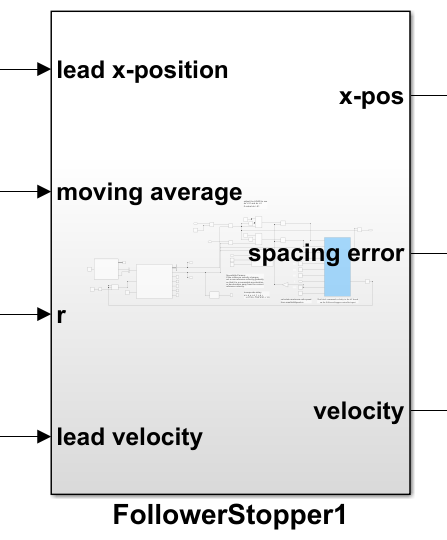
\includegraphics[width=2 in]{7carmodelblock.PNG}}
\caption{Combined AV and FollowerStopper block in Simulink.}
\label{multicarmodel1}
\end{figure}

\begin{figure}[htbp]
\centerline{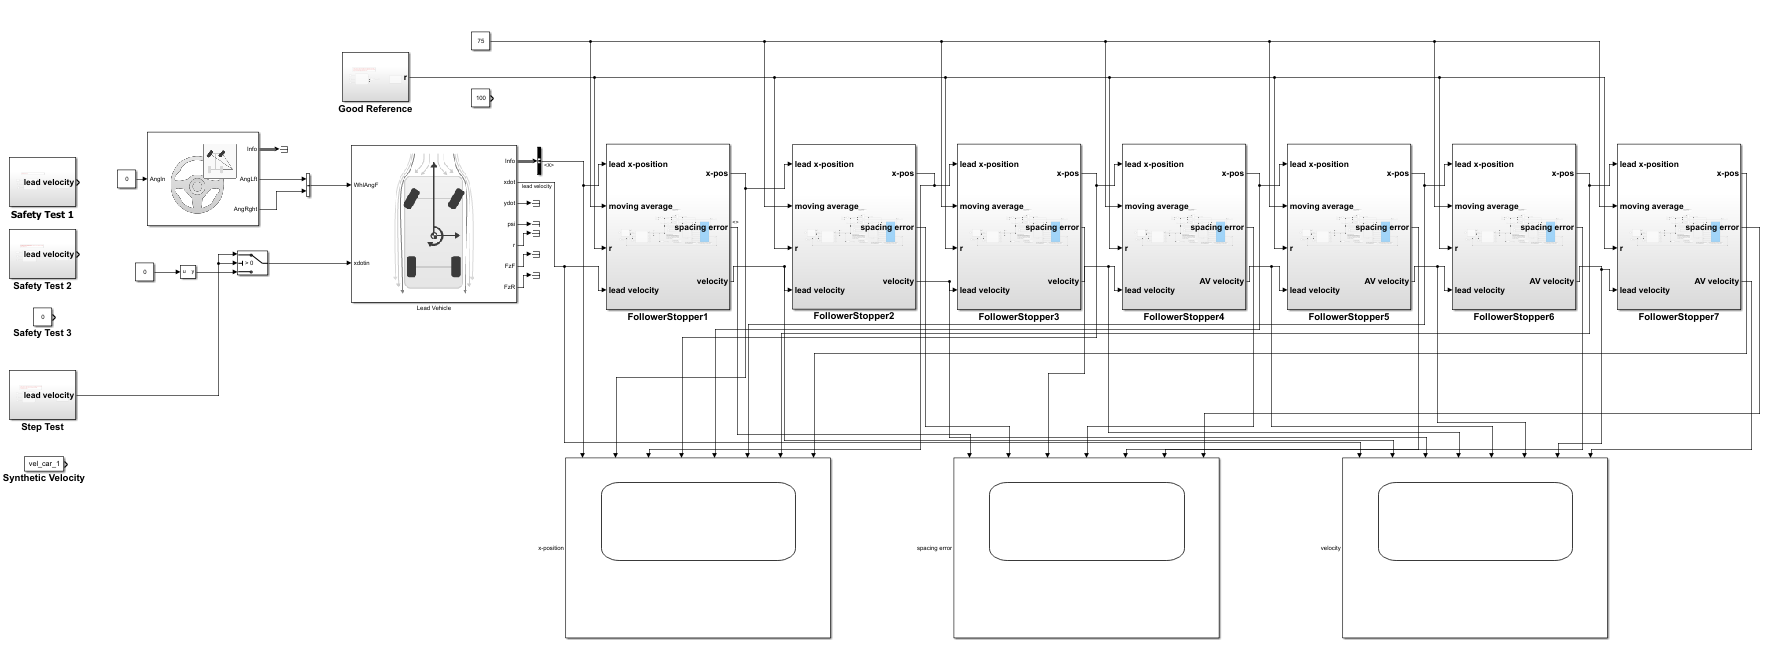
\includegraphics[width=3.5 in]{7carmodel.PNG}}
\caption{Multi-car model in Simulink.}
\label{multicarmodel2}
\end{figure}



%%%%%%%%%%%%%%%%%%%%%%%%%%%%%%%%%%%%%%%%%%%%%%%%%%%%%%%
%%%%%%%%%%%%%%%%%%%%%%%%%%%%%%%%%%%%%%%%%%%%%%%%%%%%%%%
%%%%%%%%%%%%%%%%%%%%%%%%%%%%%%%%%%%%%%%%%%%%%%%%%%%%%%%



\section{Safety and String Stability Verification}

\subsection{Safety and string stability tests}
Three tests were developed to test the safety of the original FollowerStopper and the new version of FollowerStopper, based on the optimized $\xi_j$ values. When designing the tests, the maximum speed of the AV from previous calculations was considered so that the tests would not operate above this velocity. The safety of a controller is determined by its minimum relative distance. In a worst-case scenario, FollowerStopper would have an incredible high reference velocity, so all safety tests were recorded using a relative velocity of $r=100$ m/s. Step Test was performed with a good and a bad reference velocity, as the reference velocity has an effect on the level of string stability. The safety tests used the two-car Simulink model with the original and new version of FollowerStopper while the string stability tests required a seven-car Simulink model and used only the new version of FollowerStopper.
\subsubsection{Safety Test 1}
The front of the lead vehicle starts 10 m in front of the AV. At the start of the simulation it accelerates from 0 to 12 m/s at an acceleration of $a_{max}$. It continues traveling at 12 m/s for 40 seconds. It then decelerates to 0 at a deceleration of $G$.
\subsubsection{Safety Test 2}
The front of the lead vehicle starts 10 m in front of the AV. At the start of the simulation it accelerates from 0 to 10 m/s at an acceleration of $a_{max}$. It continues traveling at 10 m/s for 25 seconds. It then accelerates at an acceleration of $a_{max}$ for $\delta=1.508$ seconds. It then immediately decelerates to 0 at a deceleration of $G$.
\subsubsection{Safety Test 3}
The front of the lead vehicle starts 1000 m in front of the AV. The lead vehicle remains stationary through the entire test.
\subsubsection{Step Test}
The front of the lead vehicle starts 10 m in front of the AV. At the start of the simulation it accelerates to 10 m/s at an acceleration of $G$. The lead continues traveling at 10 m/s for 175 seconds. It then decelerates to 2 m/s at a deceleration of $G$. It continues traveling at 2 m/s for 150 seconds. It then accelerates to 10 m/s and continues traveling at 10 m/s for the remainder of the test.

\subsection{Determination of the moving average}
Before performing the safety and string stability tests, an ideal moving average value needed to be chosen for the new FollowerStopper. To decide, Step Test was implemented using the seven-car model. The moving average was modified in each run, using no moving average, a moving average of 5, 25, 50, 75, and 100. The plots of each are detailed in Figures \ref{ma1}--\ref{ma100}, respectively, in section C of the Appendix.

In order to have individual vehicle stability, the actual relative distance must approach the desired relative distance as time approaches infinity if the lead travels at a constant velocity. Because FollowerStopper is operating at a velocity lower than the reference velocity, the desired relative distance is $\xi_2$. The plots of FollowerStopper with no moving average, a moving average of 5, 25, and 50 reveal that the velocities never reach a steady value, meaning that the relative distance would not be constant, so FollowerStopper in such cases would not be individual vehicle stable.

The plots of the moving average of 75 and 100 both reveal individual vehicle stability, but the moving average of 100 results in slight oscillations in the last vehicle at around 400 seconds, so a moving average of 75 was chosen.

\subsection{Safety verification of the original FollowerStopper}
The original $\xi_j$ values for FollowerStopper were not optimized but were merely chosen to achieve some desired behavior \cite{bhadani2019real}. Though the original FollowerStopper is safe in some instances, it is not always safe, making it a non-viable option for commercial use. In Safety Test 1, the relative distance drops to -0.7 m. In Safety Test 2, the relative distance drops to -5.7 m. In Safety Test 3, the relative distance drops to -162.3 m. In all three tests, the relative distance is negative, meaning that implementation of the original FollowerStopper results in a crash and is unsafe. The plots of the three tests are detailed Figures \ref{oldsafe1}--\ref{oldsafe3} in section D of the Appendix.

\subsection{Safety verification of the new FollowerStopper}
Due to the derivations for $\xi_j$ as detailed in section 4, the new FollowerStopper is designed for safety. In Safety Test 1, the relative distance drops to 6.6 m. In Safety Test 2, the relative distance drops to 5.6 m. In Safety Test 3, the relative distance drops to 5.0 m. In all three tests, the minimum relative distance $\Delta x>0$, so the new implementation of FollowerStopper will not result in a crash and is safe. The plots of the three tests are detailed in Figures \ref{newsafe1}--\ref{newsafe3} in section D of the Appendix.

\subsection{String stability verification}
Based on the description of string stability in the definitions section, we can test for string stability based on the AV velocity and spacing error. To test using velocities, during acceleration or deceleration or the lead, the acceleration of each successive FollowerStopper vehicle should be less extreme in order to be string stable, and the velocities should not overshoot. Additionally, velocity perturbations should dissipate with each successive car. This means that if there is a deceleration from 10 m/s to 5 m/s, each vehicle should decelerate at values decreasing in magnitude, and no vehicle should travel slower than 5 m/s at any point. 

Another way to test for string stability is based on spacing error, or the difference between the actual relative distance and desired relative distance. Because FollowerStopper is designed to follow at a distance of $\xi_2$ when the reference velocity is greater than the lead velocity, we can treat $\xi_2$ as the desired relative distance. During acceleration or deceleration, the maximum spacing error should decrease as each vehicle reacts to the change in velocity. The Step Test was performed using a bad reference velocity of $r=100$ m/s and a good reference velocity. In a real traffic-wave, a lead vehicle would slow down from its original velocity, and after exiting the wave, it would speed up back to its original velocity. The good reference velocity is designed to dissipate the traffic-wave of the Step Test. Therefore, the reference velocity is 6.1 m/s for 327 s, at which point the first AV behind the lead will catch up to the lead. At exactly this instant, the lead begins to accelerate up to 10 m/s, so the reference velocity increases to 10 m/s. In such a case, the autonomous vehicles travel at a constant velocity and never have to decelerate.

Figure \ref{stringvelbad} displays the velocities of the lead and six FollowerStopper followers with a bad reference velocity. Each successive car accelerates and decelerates with a smaller magnitude, and no car overshoots 10 m/s or 2 m/s, suggesting string stability. Figure \ref{stringvelgood} displays the velocities of the lead and six FollowerStopper followers with a good reference velocity. Though there is no overshoot, small perturbations in the first couple of FollowerStopper vehicles amplifies so that the last FollowerStopper has considerable oscillations in its velocity, suggesting string instability. 

Figure \ref{stringerrorbad} displays the spacing errors of the lead and six FollowerStopper followers with a bad reference velocity. Particularly in the middle region, each successive vehicle. has a decreasing spacing error. Though there are some wayward data points at the beginning of the data corresponding to the second acceleration in the Step Test, the data shows a similar trend of a decreasing spacing error with each successive vehicle, suggesting string stability. The regions on the left and right of the plot are concerning because a string stable controller should have either all positive or all negative spacing errors for a specific acceleration or deceleration. This is not the case in the left and right regions, suggesting string instability.

Figure \ref{stringerrorgood} displays the spacing errors of the lead and six FollowerStopper followers with the good reference velocity. The left region is similar to the left region in the bad reference velocity graph, but it is smoother. The middle region, as expected, displays no deviation from the desired relative distance, as expected. The right region, however, exemplifies the magnification of small velocity perturbations that was apparent in Figure \ref{stringvelgood} at around 350 s, suggesting string instability.

Though FollowerStopper demonstrates some qualities of string stability, the current version cannot be considered string stable because of its magnification of small perturbations of velocity. Though it seems to dissipate larger velocity changes such as from the lead, it fails to dissipate smaller changes, demonstrated particularly well by the oscillations that grow at around 50 seconds in Figure \ref{stringsafety1}, which implements Safety Test 1 on the seven-car model. If the small perturbations were to be dissipated, a more convincing case could be made for the string stability of FollowerStopper. This could be achieved through the design of a more successful command velocity filter than the current moving average filter, but this could be developed in future work.



%%%%%%%%%%%%%%%%%%%%%%%%%%%%%%%%%%%%%%%%%%%%%%%%%%%%%%%
%%%%%%%%%%%%%%%%%%%%%%%%%%%%%%%%%%%%%%%%%%%%%%%%%%%%%%%
%%%%%%%%%%%%%%%%%%%%%%%%%%%%%%%%%%%%%%%%%%%%%%%%%%%%%%%



\section{Results}

\subsection{Gazebo implementation}
Using Robot Operating Systems (ROS), the Simulink model could be downloaded as C/C++ code to be implemented in the physics-based simulator Gazebo. Gazebo operates using a hardware in the loop (HIL) principle with the CAT Vehicle, allowing for accurate estimation of implementation of FollowerStopper onto the real vehicle. When converting the Simulink model to C/C++ code, the vehicle dynamics blocks and all artificial delays were removed because the CAT Vehicle will introduce its own delays.

\subsection{CAT Vehicle testing}
Using the CAT Vehicle, we tested the new FollowerStopper controller in a parking lot owned by the University of Arizona with minimal pedestrian or vehicle traffic. A human-driven vehicle traveled at a slow velocity, acceleration, and deceleration, and the CAT Vehicle successfully and safely reacted to the input. Subsequently, a human moved in front of the vehicle at a walking pace while making several stops along the way, and the vehicle safely followed without any driver input to the gas or brake pedals. No conclusions about string stability could be made during the physical tests because such conclusions can only be tested with several autonomous vehicles with FollowerStopper. Unfortunately, there is only one CAT Vehicle, limiting string stability testing.



%%%%%%%%%%%%%%%%%%%%%%%%%%%%%%%%%%%%%%%%%%%%%%%%%%%%%%%
%%%%%%%%%%%%%%%%%%%%%%%%%%%%%%%%%%%%%%%%%%%%%%%%%%%%%%%
%%%%%%%%%%%%%%%%%%%%%%%%%%%%%%%%%%%%%%%%%%%%%%%%%%%%%%%



\section{Conclusion}
In this paper we present an optimized version of the velocity controller FollowerStopper using theoretical proof, Simulink simulation, and implementation onto the CAT Vehicle autonomous vehicle. The development of the optimization and development of the Simulink model, which served as the primary platform for testing, were discussed rigorously. The original version of FollowerStopper proved useful in avoiding crashes and dissipating traffic waves in previous experiments setup through the University of Arizona. We provide a formal analysis of the safety and string stability of the velocity controller.

The physics-based proof demonstrates that FollowerStopper should never crash theoretically, and a variety of tests with the Simulink model asserts this claim. Some tests in Simulink demonstrate string stability, while others provide contradictions. FollowerStopper possesses qualities of string stability through its dissipation of the synthetically-created vehicle velocity data, but it amplifies small velocity perturbations that it creates on its own, resulting in a conclusive determination that the optimized version is not string stable.

\subsection{Future work}
Of upmost concern is modifying FollowerStopper to maintain its safety but also to be string stable. Development of a more extensive command velocity filter than just a moving average could dissipate the small perturbations, resulting in a string stable controller.

Little work was done to optimize the reference velocity $r$. An idea could be to use smart phone traffic congestion data to calculate the length of a traffic wave and average speed of the vehicles in the wave as a reference velocity for the autonomous vehicle.

FollowerStopper was proven to be safe given dry, sunny conditions when the car is traveling straight with no incline. Future research could be done to edit the acceleration parameters based on the incline of the road, the weather conditions, and the wear of the tire. \cite{muller2003estimation} shows that different weather conditions dramatically affect the coefficient of tire-road friction.

The current Simulink model has several limitations. The most concerning limitation is its difficulty in handling the AV velocity delay. Future work could attempt to use a different vehicle dynamics model or an entire new platform that could better incorporate delay. 

Use of LiDAR as the main sensor input is limiting due to the short range of LiDAR. Future work could test the accuracy and usability of relying on radar or some other longer-range sensor so that the vehicle can safely travel faster than the current maximum speed of $v_{AVsafe}=13.69$ m/s. A redevelopment of $\xi_2$ to a lesser value could also increase the maximum speed.



%%%%%%%%%%%%%%%%%%%%%%%%%%%%%%%%%%%%%%%%%%%%%%%%%%%%%%%
%%%%%%%%%%%%%%%%%%%%%%%%%%%%%%%%%%%%%%%%%%%%%%%%%%%%%%%
%%%%%%%%%%%%%%%%%%%%%%%%%%%%%%%%%%%%%%%%%%%%%%%%%%%%%%%
%%%%%%%%%%%%%%%%%%%%%%%%%%%%%%%%%%%%%%%%%%%%%%%%%%%%%%%
%%%%%%%%%%%%%%%%%%%%%%%%%%%%%%%%%%%%%%%%%%%%%%%%%%%%%%%
%%%%%%%%%%%%%%%%%%%%%%%%%%%%%%%%%%%%%%%%%%%%%%%%%%%%%%%


\bibliography{citations}
\bibliographystyle{ieeetr}
\vspace{12pt}



%%%%%%%%%%%%%%%%%%%%%%%%%%%%%%%%%%%%%%%%%%%%%%%%%%%%%%%
%%%%%%%%%%%%%%%%%%%%%%%%%%%%%%%%%%%%%%%%%%%%%%%%%%%%%%%
%%%%%%%%%%%%%%%%%%%%%%%%%%%%%%%%%%%%%%%%%%%%%%%%%%%%%%%



\onecolumn
\begin{appendix}

\subsection{Determination of the maximum deceleration of the lead vehicle}
To determine the maximum deceleration of the lead vehicle, consider Figure \ref{fig3}.

\begin{figure}[htbp]
\centerline{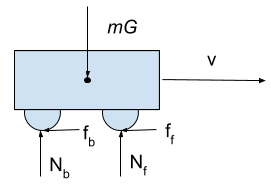
\includegraphics[width=2.00 in]{maxDecel.PNG}}
\caption{Free-body diagram of a four-wheeled vehicle during deceleration.}
\label{fig3}
\end{figure}

Given the mass, $m$, of the vehicle and acceleration due to gravity, $G$, the normal force acting on the front and back tires can be expressed
\begin{eqnarray*}
mG=N_f+N_b=N.
\end{eqnarray*}
The force of friction is proportional to the normal force by means of the coefficient of friction, $\mu$. Assuming that the force of friction on the front and back tires is equal,
\begin{eqnarray*}
f_f+f_b=N_f\mu+N_b\mu=(N_f+N_b)\mu=N\mu=mG\mu
\end{eqnarray*}
According to Newton's second law, the sum of the forces is proportional to the mass and the acceleration of an object. If we only consider the car's longitudinal direction, or the direction in which it is traveling at velocity, $v$,
\begin{eqnarray*}
\sum F &=& ma \\
-f_f-f_b &=& ma \\
-mG\mu &=& ma \\
a &=& -G\mu
\end{eqnarray*}




\subsection{Derivation of $\xi_1$}

\begin{figure}[htbp]
\centerline{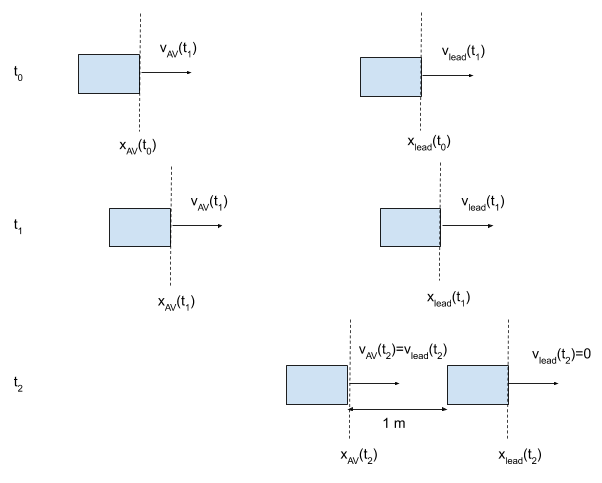
\includegraphics[width=6 in]{xiDerivation.PNG}}
\caption{Emergency breaking progression.}
\label{fig2}
\end{figure}

Consider Figure \ref{fig2}, depicting two cars at times $t_0$, $t_1$, and $t_2$. $t_0$ is the time at which the relative distance is equal to the emergency breaking distance, that is, $\Delta x(t_0)=\xi_1$. $t_1$ occurs $\delta$ seconds after reaching $\xi_1$, at which point the AV will first be able to react to being within the emergency breaking distance due to the delay. $t_2$ is the time at which both vehicles will be stopped and the AV will be a distance $\psi$ behind the lead vehicle. The vehicle to the left is the AV and the vehicle to the right is the human-driven lead. All positions and velocities have been labeled as functions of time, and the relative positions and relative velocities at each time can be computed according to the equations in section II.A. First we will consider the motion of the two vehicles from time $t_1$ to time $t_2$. Within this time region in a worst-case scenario, both the AV and lead will constantly decelerate at their maximum decelerations, and in the derivation we will express the lead vehicle maximum deceleration as proportional to the AV maximum deceleration with proportionality constant $k$. That is, suppose $ka_{dmax}$ is the maximum deceleration of the lead. The minimum distance $\Delta x(t_1)$ which can be considered safe will assume that the AV will end up at a relative distance $\Delta x(t_2)= \psi$ from the lead vehicle. The following derivation uses this idea with the equations of motion to derive a value for $\Delta x(t_1)$.

\begin{eqnarray*}
{\rm Equation\ of\ motion:\ } v^2-v_0^2 = 2a\Delta x \\
{\rm Lead\ vehicle:\ } \\
v_{lead}(t_2)^2-v_{lead}(t_1)^2 &=& 2 ka_{dmax}(x_{lead}(t_2)-x_{lead}(t_1)) \\
0-v_{lead}(t_1)^2 &=& 2ka_{dmax}x_{lead}(t_2)-2ka_{dmax}x_{lead}(t_1)) \\
2a_{dmax}x_{lead}(t_1) -{v_{lead}(t_1)^2\over k} &=& 2a_{dmax}x_{lead}(t_2) \\
{\rm Autonomous\ vehicle:\ } \\
v_{AV}(t_2)^2-v_{AV}(t_1)^2 &=& 2 a_{dmax}(x_{AV}(t_2)-x_{AV}(t_1)) \\
0-v_{AV}(t_1)^2 &=& 2a_{dmax}(x_{lead}(t_2)-l_{lead}-\psi-x_{AV}(t_1)) \\
2a_{dmax}(l_{lead}+\psi+x_{AV}(t_1))-v_{AV}(t_1)^2 &=& 2a_{dmax}x_{lead}(t_2)\\
{\rm Setting\ the\ equations\ equal:} \\
2a_{dmax}x_{lead}(t_1) -{v_{lead}(t_1)^2\over k} &=& 2a_{dmax}(l_{lead}+\psi+x_{AV}(t_1))-v_{AV}(t_1)^2 \\
2a_{dmax}(x_{lead}(t_1)-x_{AV}(t_1)-l_{lead}) &=& 2a_{dmax}\psi+{v_{lead}(t_1)^2\over k}-v_{AV}(t_1)^2\\
\Delta x(t_1) &=& \psi+{1\over 2a_{dmax}}({v_{lead}(t_1)^2\over k}-v_{AV}(t_1)^2) \\
\end{eqnarray*}

Delay is an essential consideration because if the AV is currently at $\Delta x=\Delta x(t_1)$, it needs to initiate emergency breaking, but it will not do as such until $\delta$ seconds have passed, where $\delta$ is the delay of the system. Consider the time $t_0$ at which point the AV recognizes that it must send an emergency braking command in order to initiate emergency braking at the instant it reaches $t_1$ from the above example. When considering the emergency stopping distance $\xi_1$, we must plan for the worst case scenario. The worst case scenario is that at time $t_0$ the lead car begins to accelerate before coming to an immediate stop because the AV might think that it can begin to accelerate as well. Though from time $t_0$ to time $t_1$ the accelerations might fluctuate, a worst-case scenario would involve maximum acceleration of the AV and maximum deceleration of the lead. The following derivation, based off of a derivation in \cite{bhadani2019real}, incorporates the delay to determine what a safe value of $\xi_1$ will equal such that if $\Delta x=\xi_1$, the AV will initiate hard braking at exactly $\Delta x = \Delta x(t_1)$. In this setup, $\xi_1=\Delta x(t_0)$.

\begin{eqnarray*}
{\rm Equation\ of\ motion:\ } x &=& x_0 + v_0t + {1\over 2}at^2 \\
{\rm Distance\ traveled\ during\ delay : \ } \\
x_{lead}(t_1) &=& x_{lead}(t_0)+v_{lead}(t_0)\delta+{1\over 2}a_{lead}(t_0)\delta^2 \\
x_{AV}(t_1) &=& x_{AV}(t_0)+v_{AV}(t_0)\delta+{1\over 2}a_{AV}(t_0)\delta^2
\end{eqnarray*}
Worst-case scenario, $a_{lead}(t_0)=a_{dmaxLEAD}=ka_{dmax}$, $a_{AV}(t_0)=a_{max}$
\begin{eqnarray*}
{\rm Incorporating\ relative\ distance:\ } \\
\Delta x(t_1) &=& \Delta x(t_0) + (v_{lead}(t_0)-v_{AV}(t_0))\delta + {1\over 2}(ka_{dmax}-a_{max})\delta^2\\
\xi_1 = \Delta x(t_0) &=& \Delta x(t_1) - (v_{lead}(t_0)-v_{AV}(t_0))\delta - {1\over 2}(ka_{dmax}-a_{max})\delta^2\\
&=& \psi+{1\over 2a_{dmax}}({v_{lead}(t_1)^2\over k}-v_{AV}(t_1)^2) \\
&& - (v_{lead}(t_0)-v_{AV}(t_0))\delta - {1\over 2}(ka_{dmax}-a_{max})\delta^2
\end{eqnarray*}

The above equation for $\xi_1$ guarantees that a crash is impossible and that the AV will never come within 1 meter of the lead, assuming that there are no unexpected obstacles that appear between the AV and the lead. However, when the AV arrives at time $t_0$, it will not know $v_{lead}(t_1)$ or $v_{AV}(t_1)$. Both are best approximated using the equation of motion, $v=v_o+at$, with $a$ set to a safe value. In a worst-case scenario, the $v_{lead}$ will be slower than expected and $v_{AV}$ will be faster than expected. Therefore safe acceleration values will be the same as indicated in the previous derivation. Because all time-dependent values will be expressed at the same time $t_0$, the notation can be dropped, giving
\begin{eqnarray*}
\xi_1 &=& \psi+{1\over 2ka_{dmax}}((v_{lead}+ka_{dmax}\delta)^2-k(v_{AV}+a_{max}\delta)^2) - (v_{lead}-v_{AV})\delta - {1\over 2}(ka_{dmax}-a_{max})\delta^2 \\
&=& \psi+{1\over 2ka_{dmax}}(v_{lead}^2+2v_{lead}ka_{dmax}\delta+k^2a_{dmax}^2\delta^2-kv_{AV}^2-2kv_{AV}a_{cmft}\delta-ka_{cmft}^2\delta^2) \\
&& -v_{lead}\delta+v_{AV}\delta-{ka_{dmax}\delta^2\over 2}+{a_{max}\delta^2\over2} \\
&=& \psi+{v_{lead}^2\over 2ka_{dmax}}+{v_{lead}\delta}+{ka_{dmax}\delta^2 \over 2}-{v_{AV}^2\over 2a_{dmax}}-{v_{AV}a_{cmft}\delta \over a_{dmax}}-{a_{max}^2\delta^2\over 2a_{dmax}}-v_{lead}\delta+v_{AV}\delta-{ka_{dmax}\delta^2\over 2}+{a_{max}\delta^2\over2} \\
&=& \psi+{1\over 2ka_{dmax}}(v_{lead}^2-kv_{AV}^2)+v_{AV}(1-{a_{max}\over a_{dmax}})\delta+{a_{max}\over 2}(1-{a_{max}\over a_{dmax}})\delta^2.
\end{eqnarray*}

Finally, it must be noted that it is never desirable for $\xi_1$ to drop below $\psi$, the minimum acceptable relative distance. In the above equation for $\xi_1$, the first, third, and fourth terms will always be positive, but the second term could be negative. To assure that $\xi_1$ will remain greater than $\psi$, the second term must be set equal to 0 if it is negative, giving a final solution
\begin{eqnarray*}
\xi_1 &=& \psi+\Delta v^{**}+v_{AV}(1-{a_{max}\over a_{dmax}})\delta+{a_{max}\over 2}(1-{a_{max}\over a_{dmax}})\delta^2 \\
\Delta v^{**} &=& max(0,{1\over 2ka_{dmax}}(v_{lead}^2-kv_{AV}^2)).
\end{eqnarray*}


\pagebreak
\subsection{Moving average plots}
\begin{figure}[htbp!]
\centerline{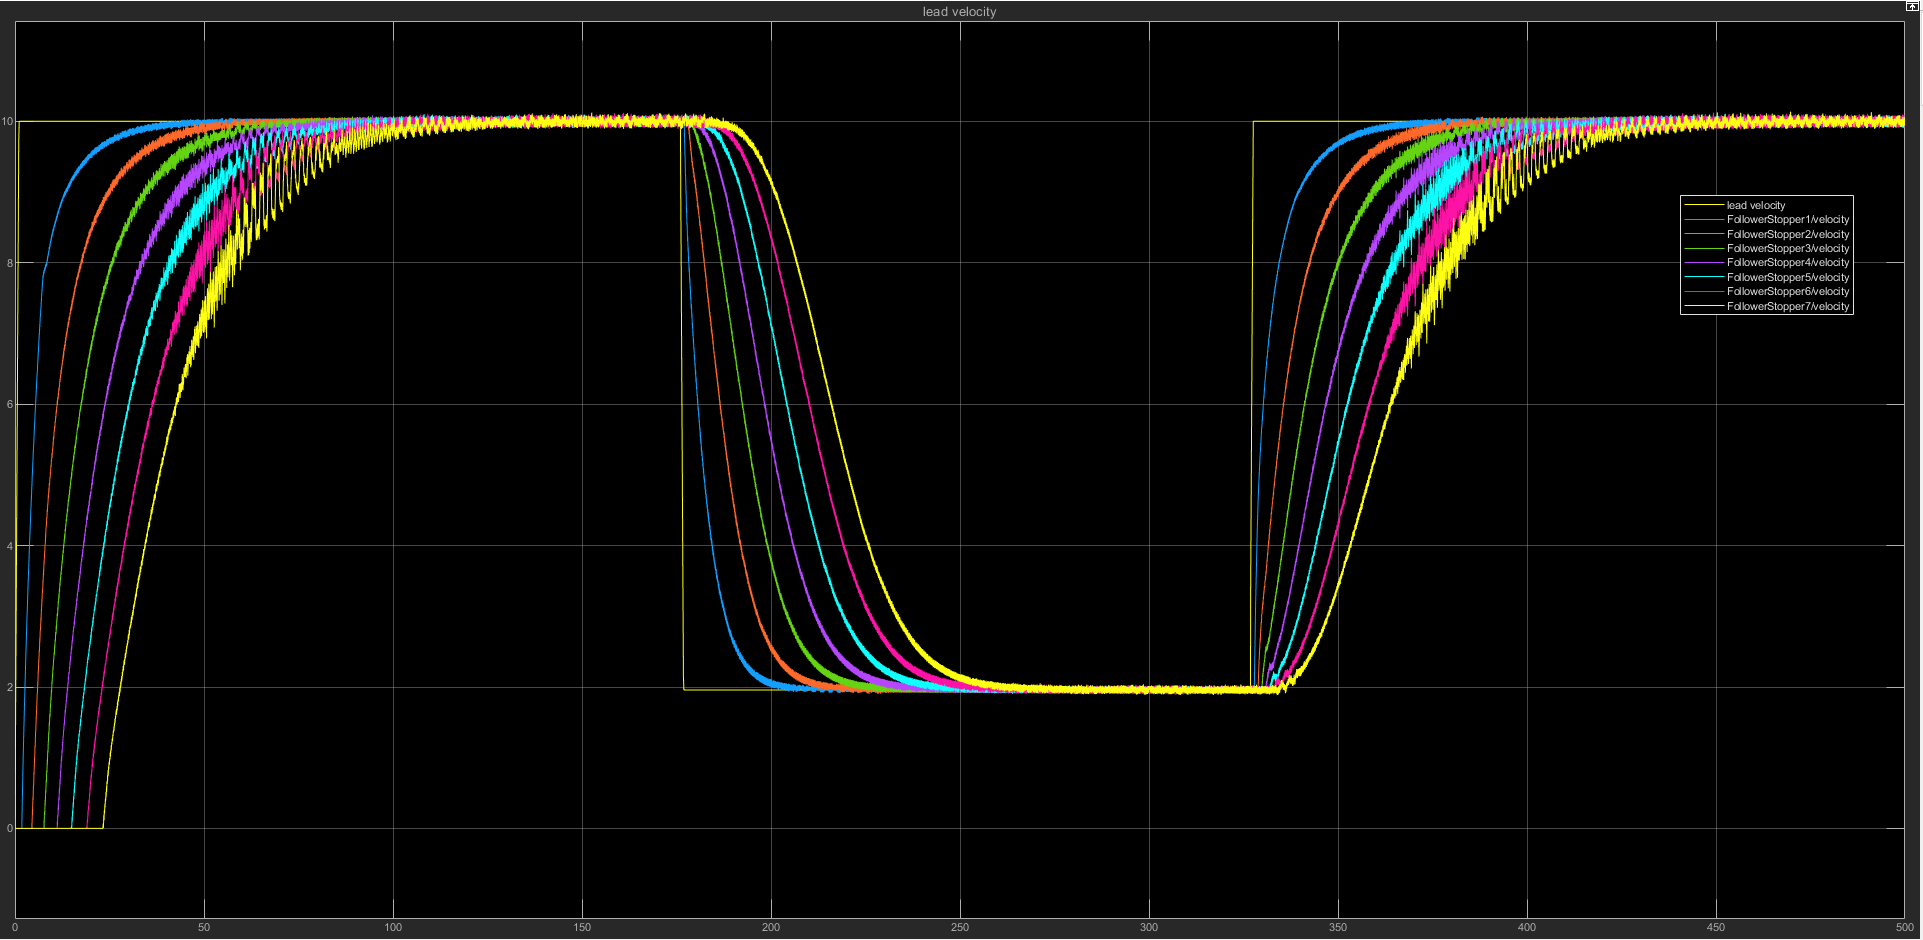
\includegraphics[width=6.50 in]{multiFS_velbad_ma1.PNG}}
\caption{Step Test with no moving average.}
\label{ma1}
\end{figure}

\begin{figure}[htbp!]
\centerline{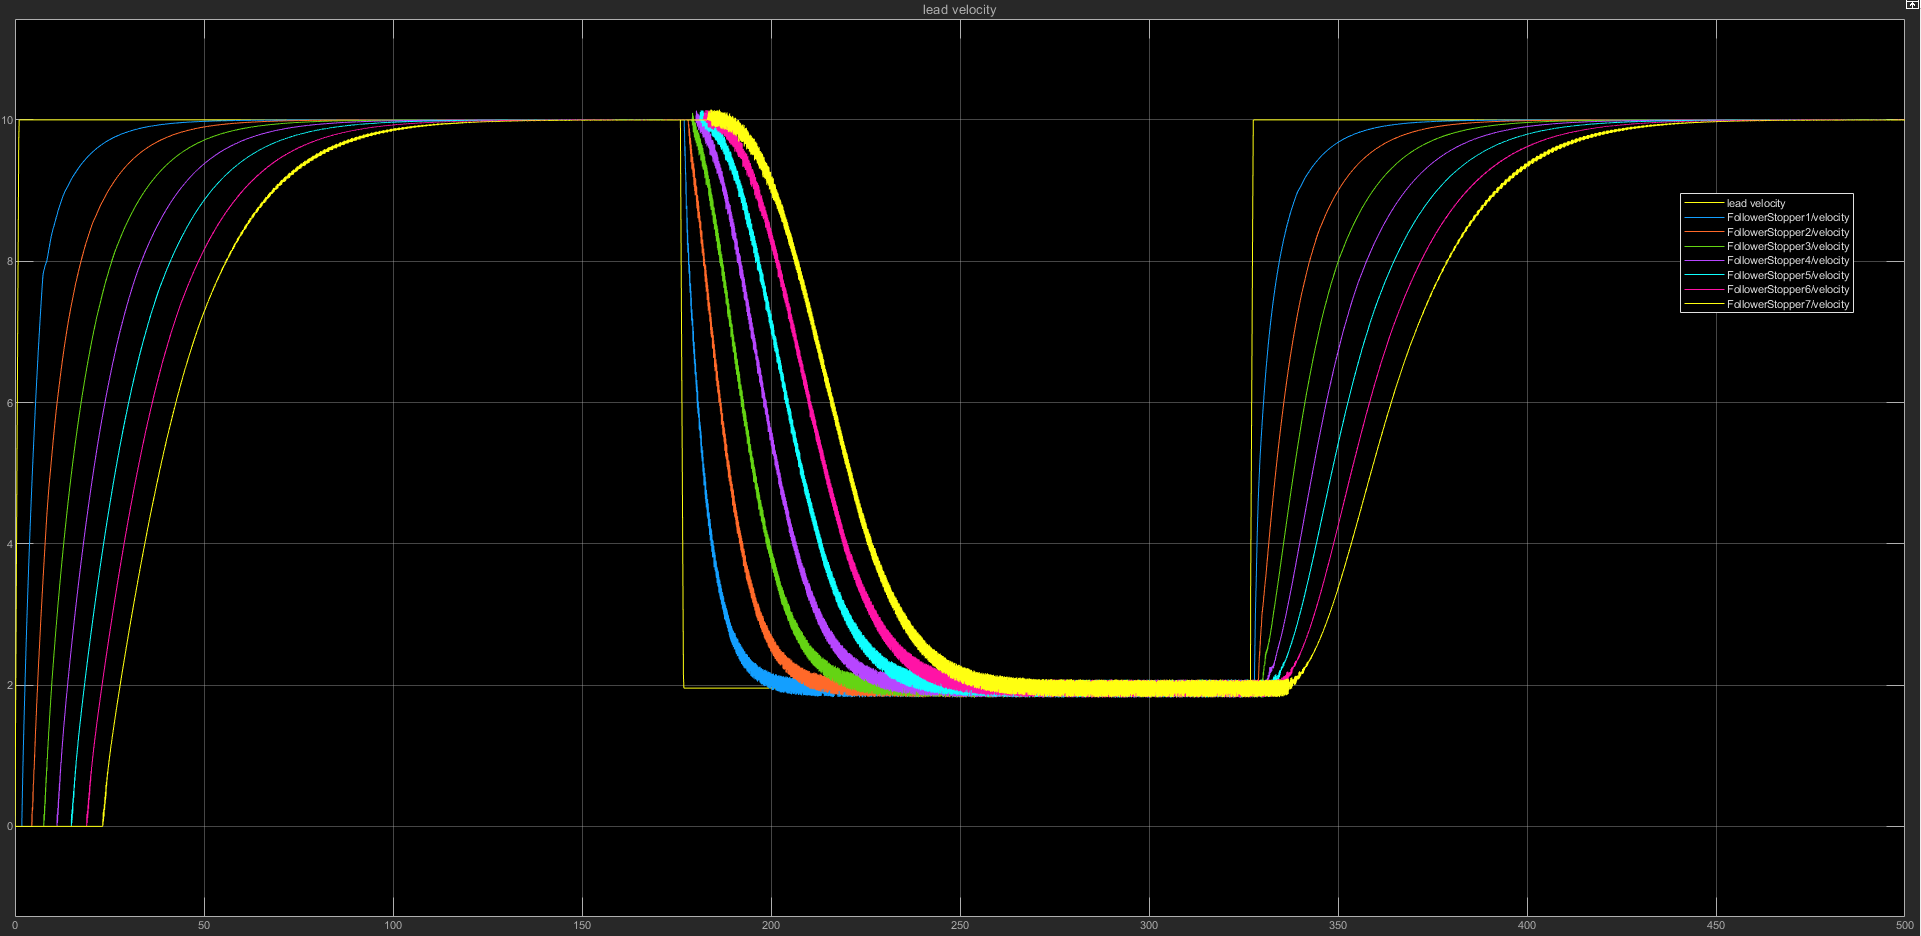
\includegraphics[width=6.50 in]{multiFS_velbad_ma5.PNG}}
\caption{Step Test with a moving average of 5.}
\label{ma5}
\end{figure}

\begin{figure}[htbp!]
\centerline{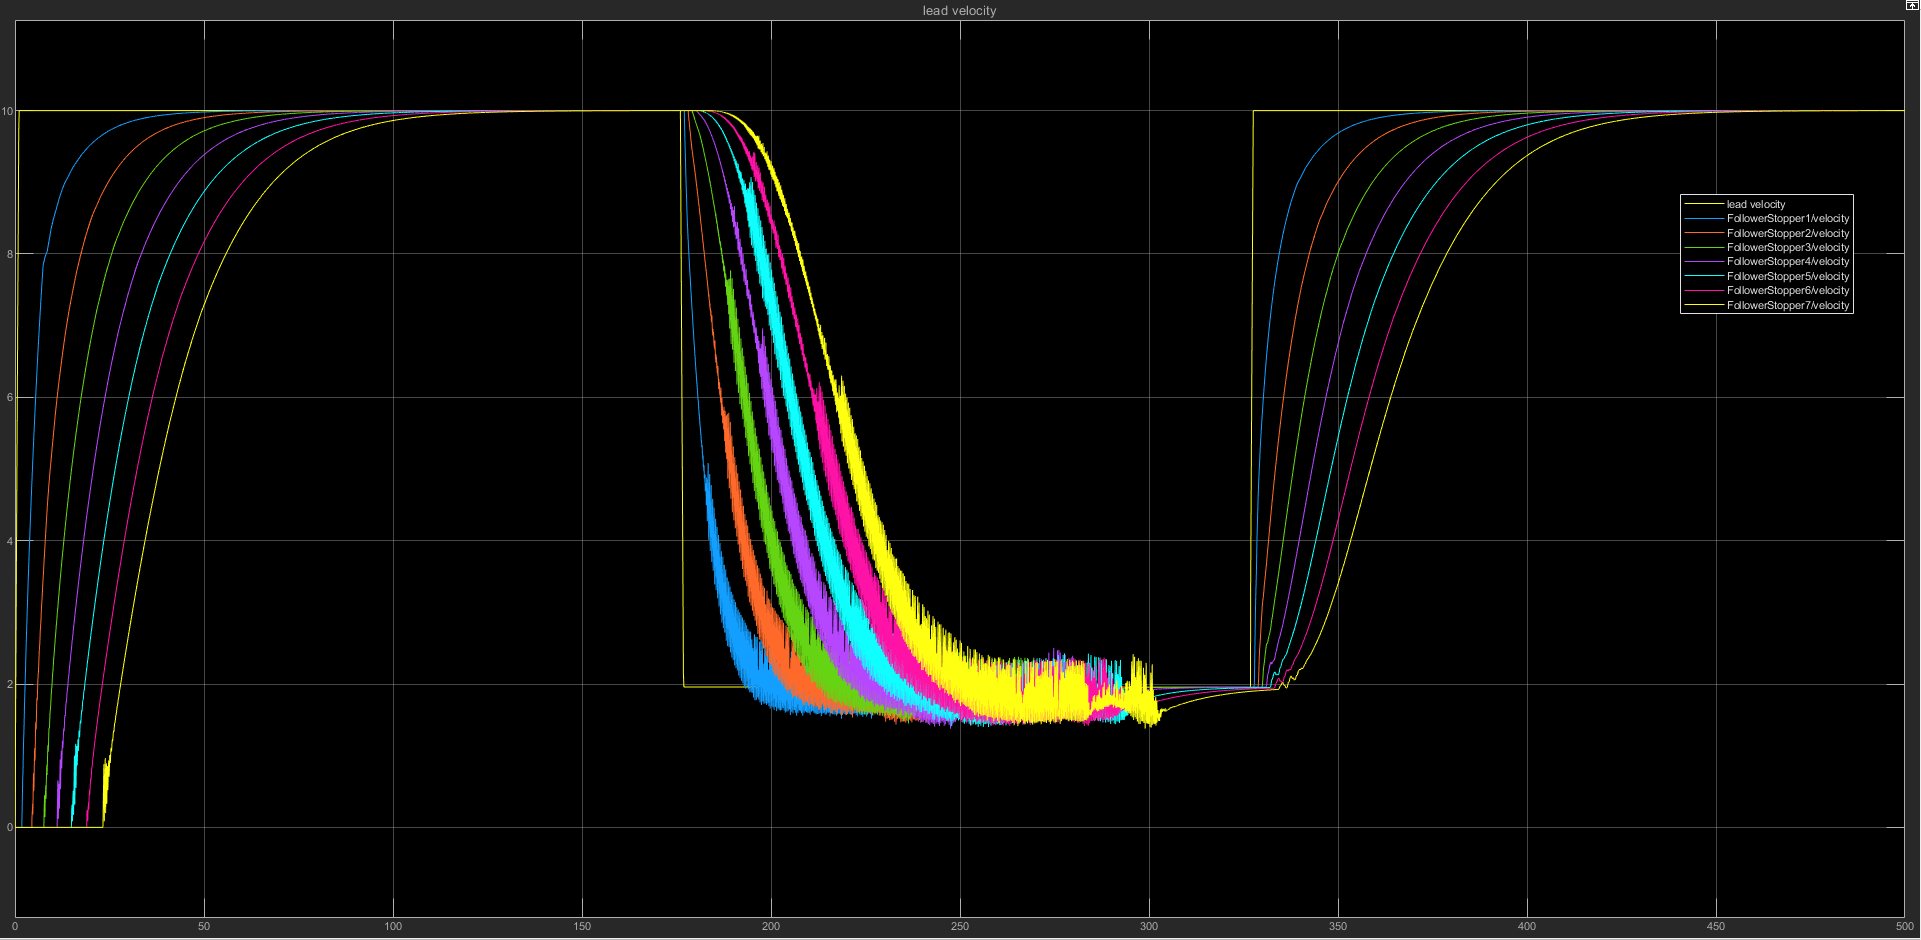
\includegraphics[width=6.50 in]{multiFS_velbad_ma25.PNG}}
\caption{Step Test with a moving average of 25.}
\label{ma25}
\end{figure}

\begin{figure}[htbp!]
\centerline{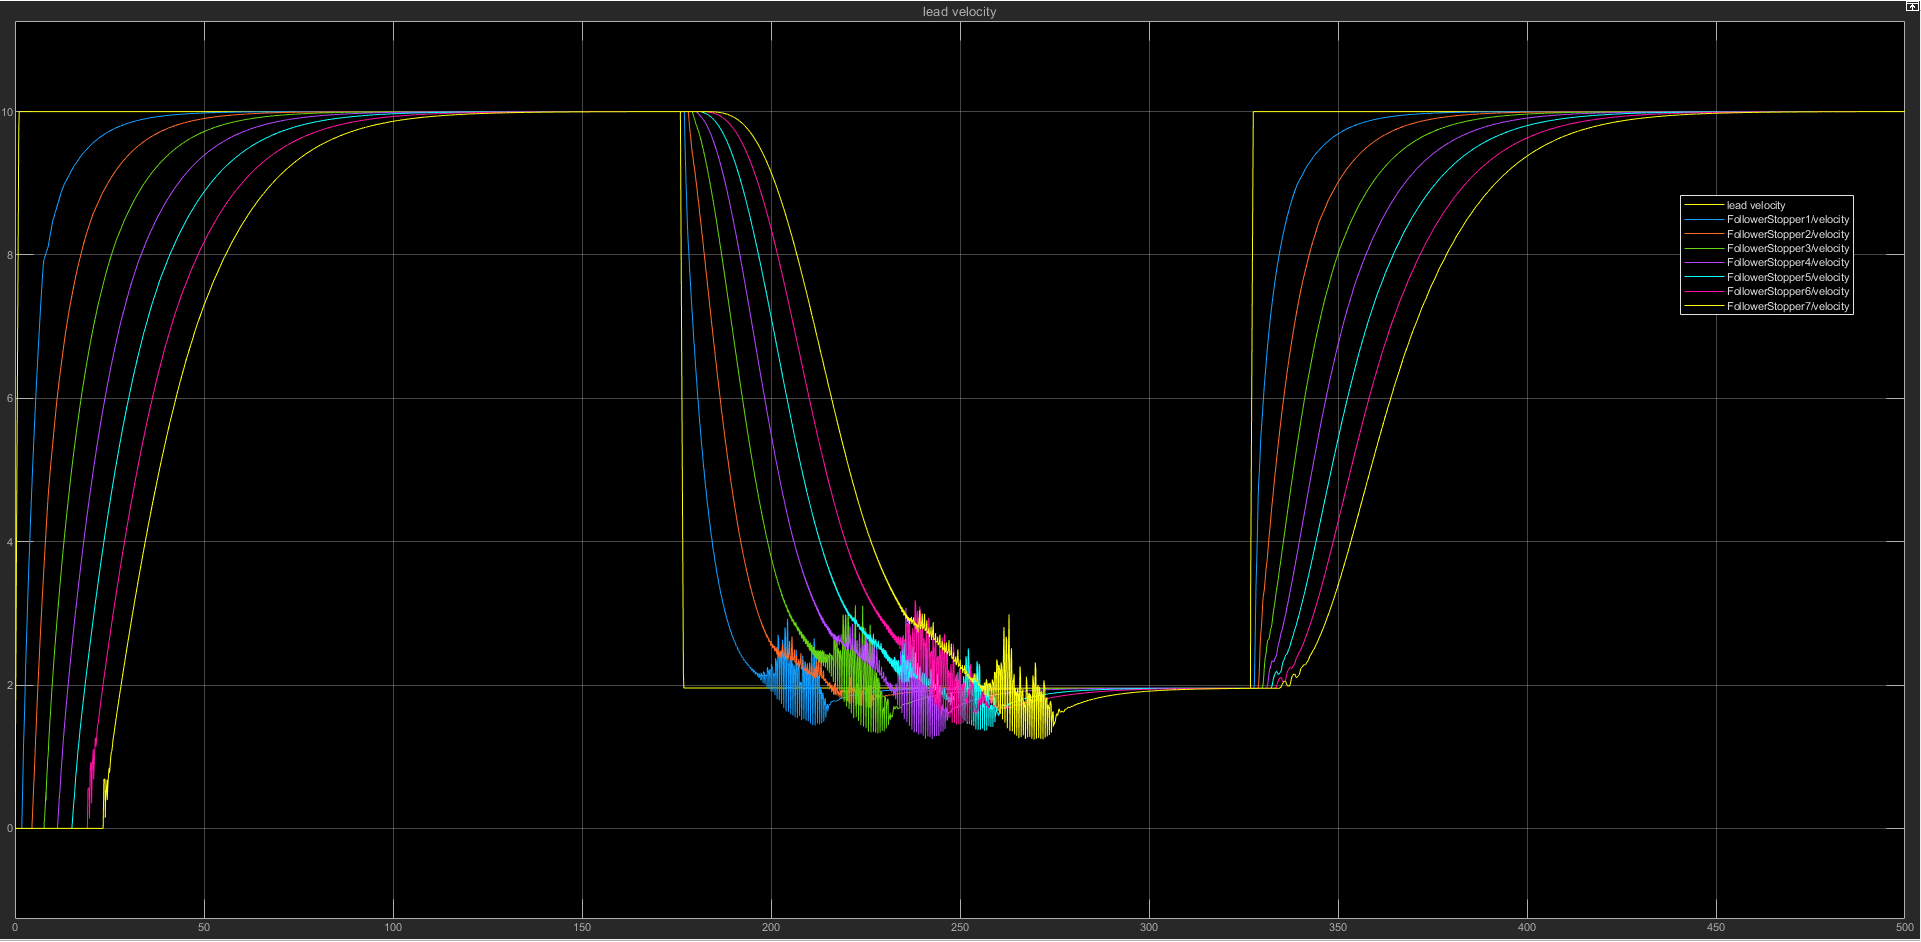
\includegraphics[width=6.50 in]{multiFS_velbad_ma50.PNG}}
\caption{Step Test with a moving average of 50.}
\label{ma50}
\end{figure}

\begin{figure}[htbp!]
\centerline{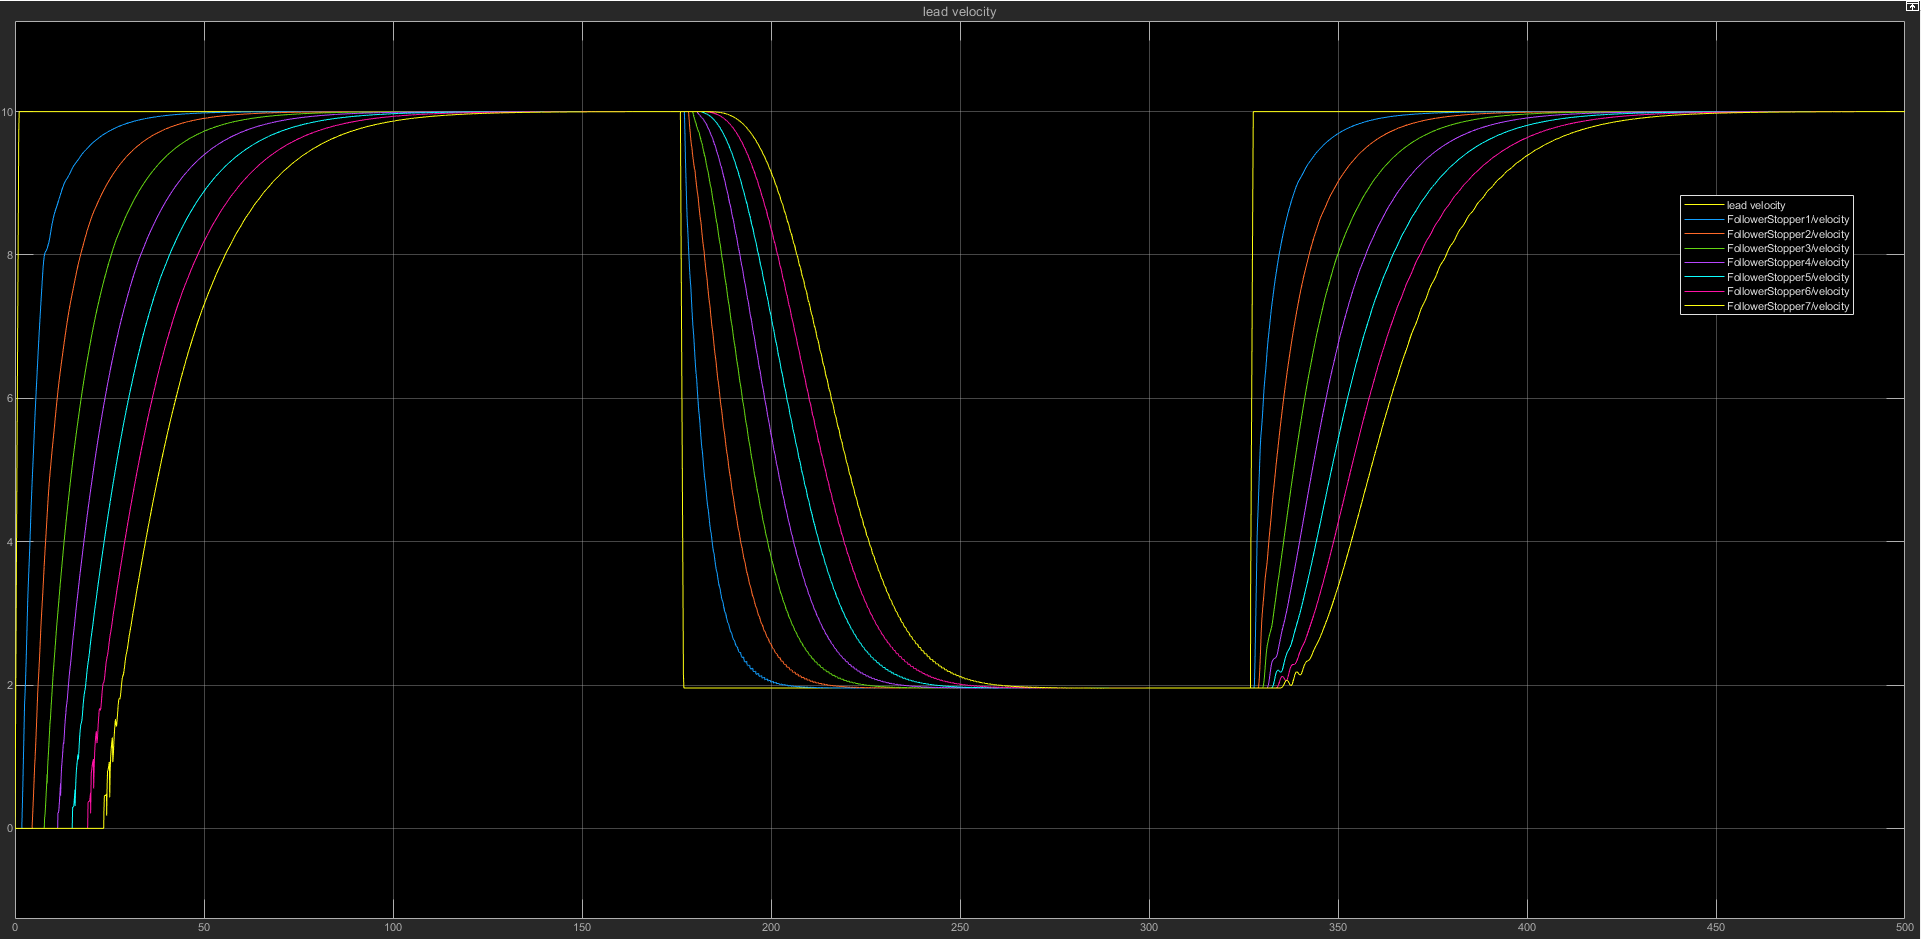
\includegraphics[width=6.50 in]{multiFS_velbad_ma75.PNG}}
\caption{Step Test with a moving average of 75.}
\label{ma75}
\end{figure}

\begin{figure}[htbp!]
\centerline{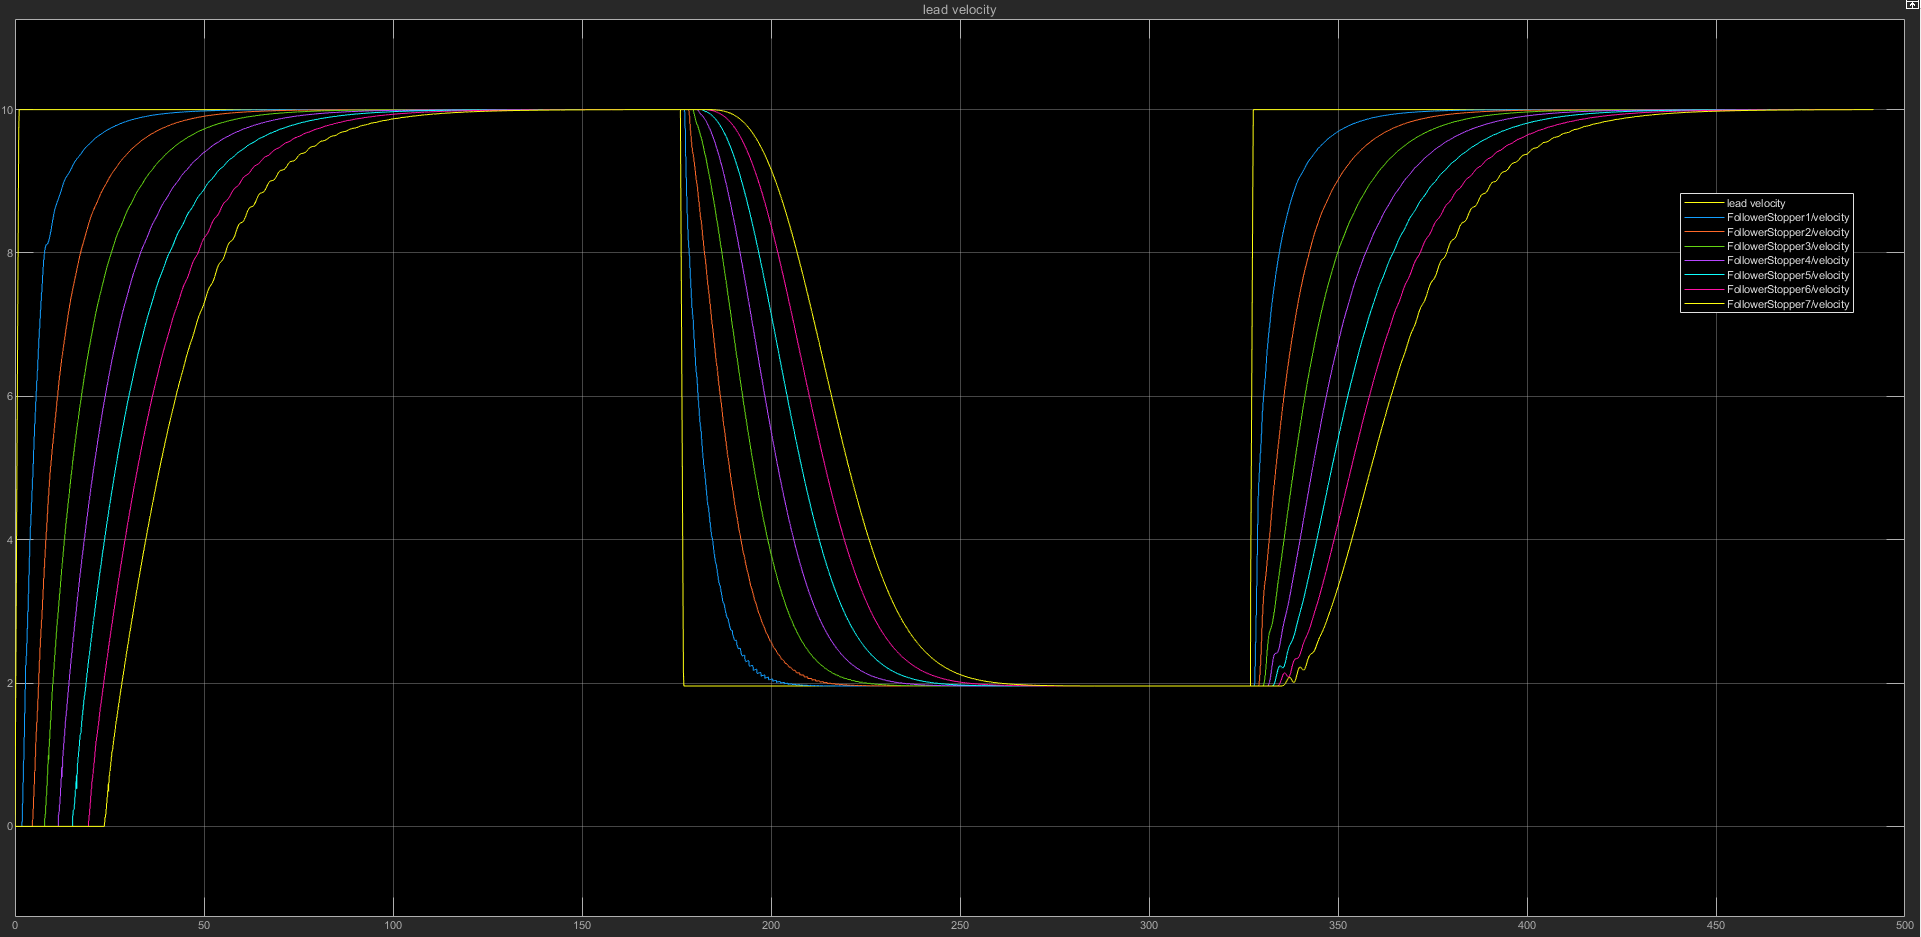
\includegraphics[width=6.50 in]{multiFS_velbad_ma100.PNG}}
\caption{Step Test with a moving average of 100.}
\label{ma100}
\end{figure}

\begin{verbatim}























\end{verbatim}
\pagebreak
\subsection{FollowerStopper safety plots}

\begin{figure}[htbp]
\centerline{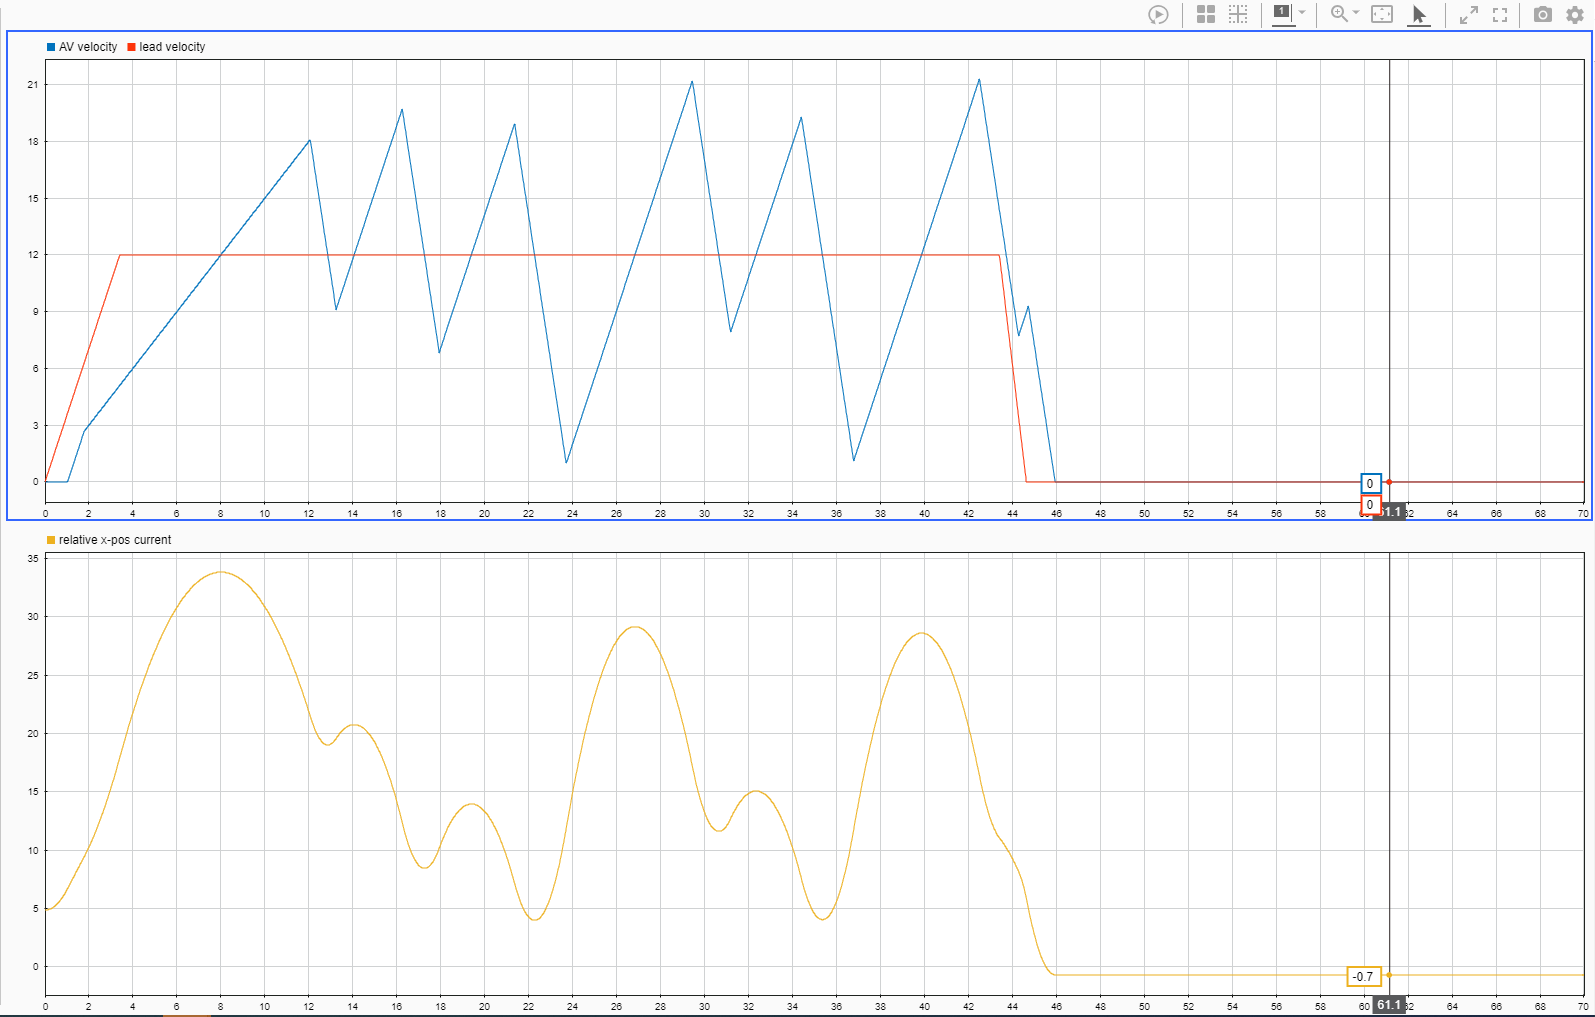
\includegraphics[width=5.71 in]{oldFS_safety1.PNG}}
\caption{Original FollowerStopper in Safety Test 1.}
\label{oldsafe1}
\end{figure}

\begin{figure}[htbp]
\centerline{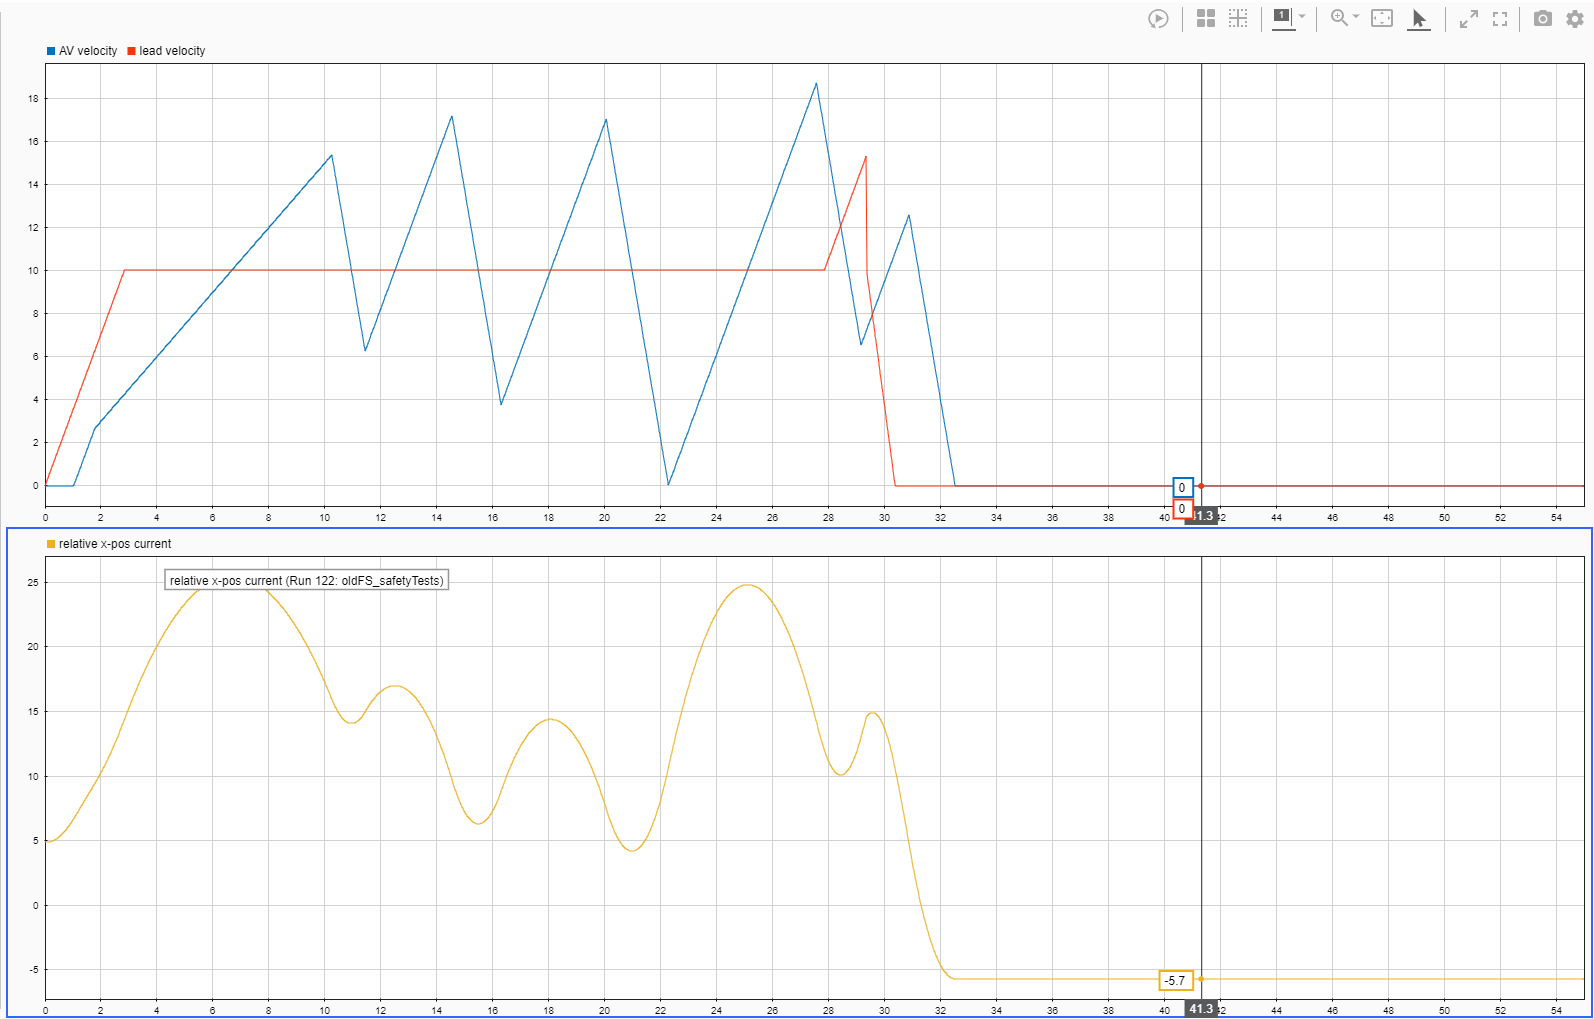
\includegraphics[width=5.71 in]{oldFS_safety2.PNG}}
\caption{Original FollowerStopper in Safety Test 2.}
\label{oldsafe2}
\end{figure}

\begin{figure}[htbp]
\centerline{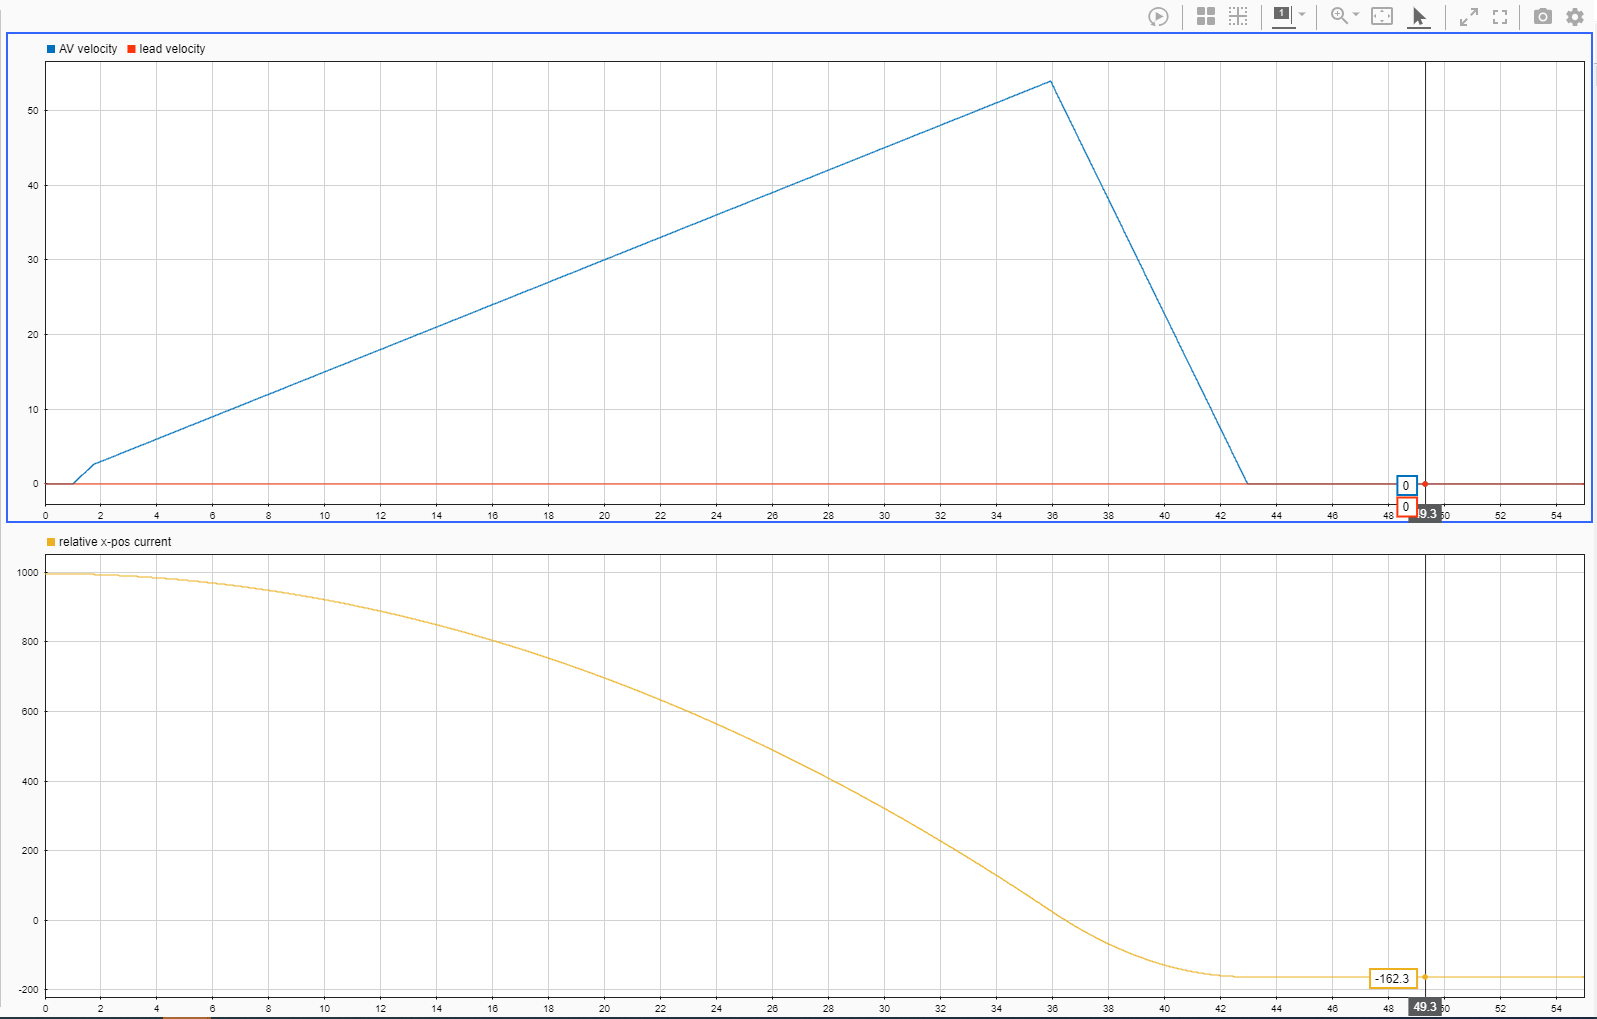
\includegraphics[width=5.71 in]{oldFS_safety3.PNG}}
\caption{Original FollowerStopper in Safety Test 3.}
\label{oldsafe3}
\end{figure}

\begin{figure}[htbp]
\centerline{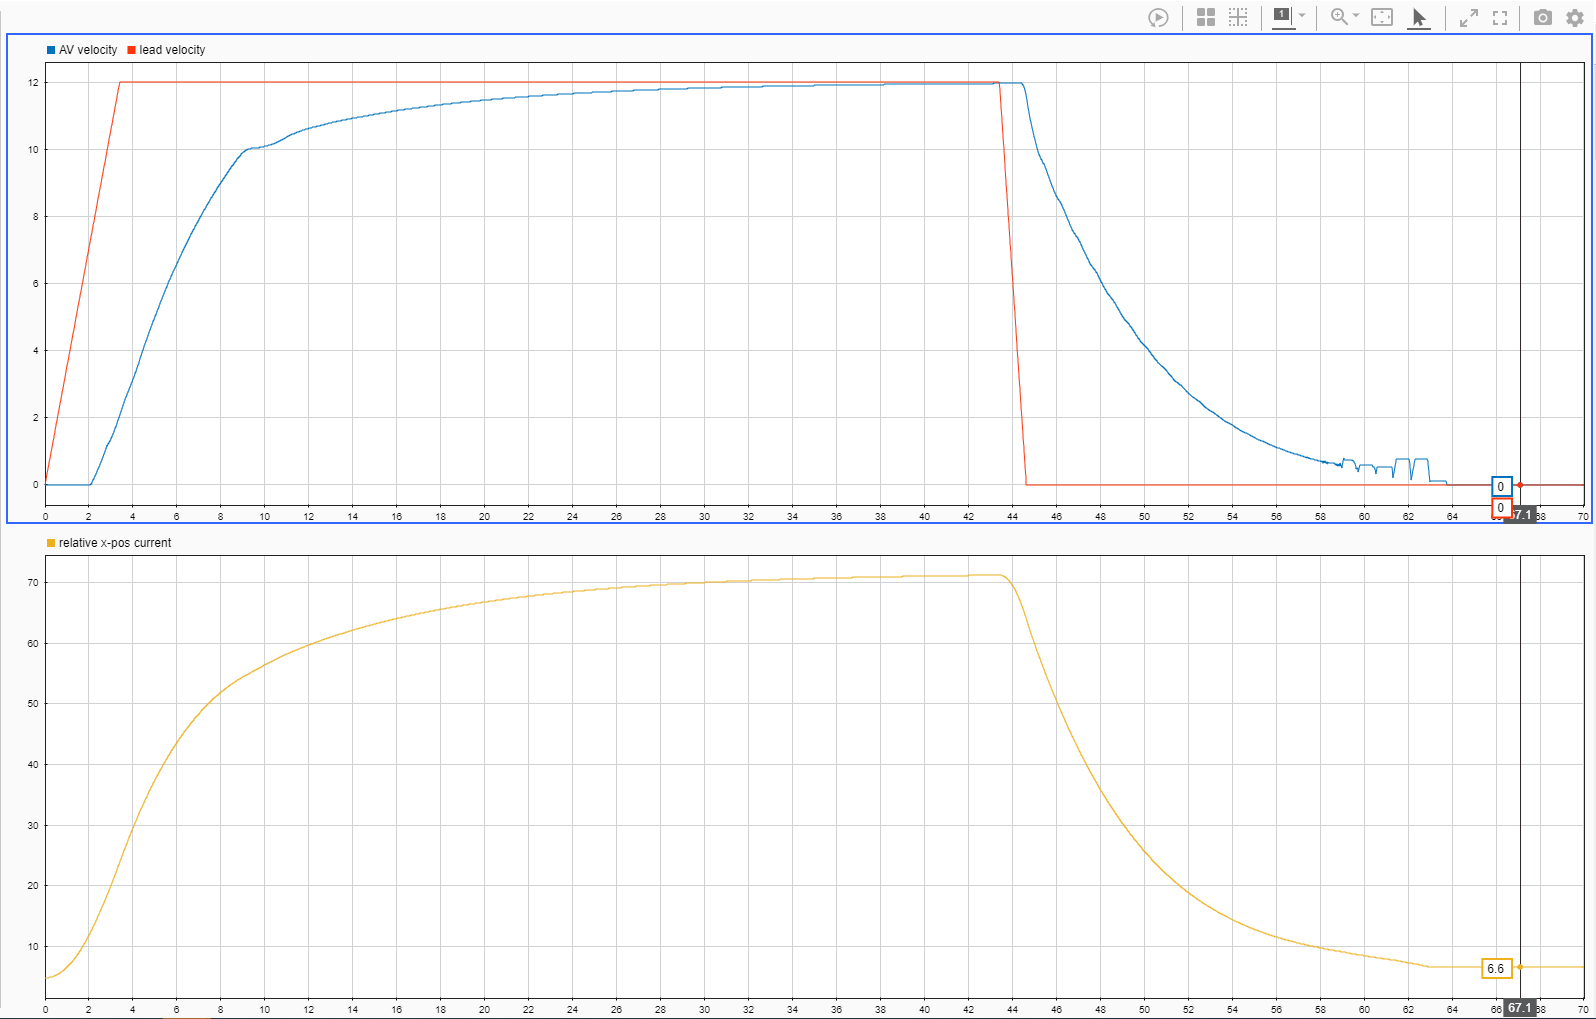
\includegraphics[width=5.71 in]{newFS_safety1.PNG}}
\caption{New FollowerStopper in Safety Test 1.}
\label{newsafe1}
\end{figure}

\begin{figure}[htbp]
\centerline{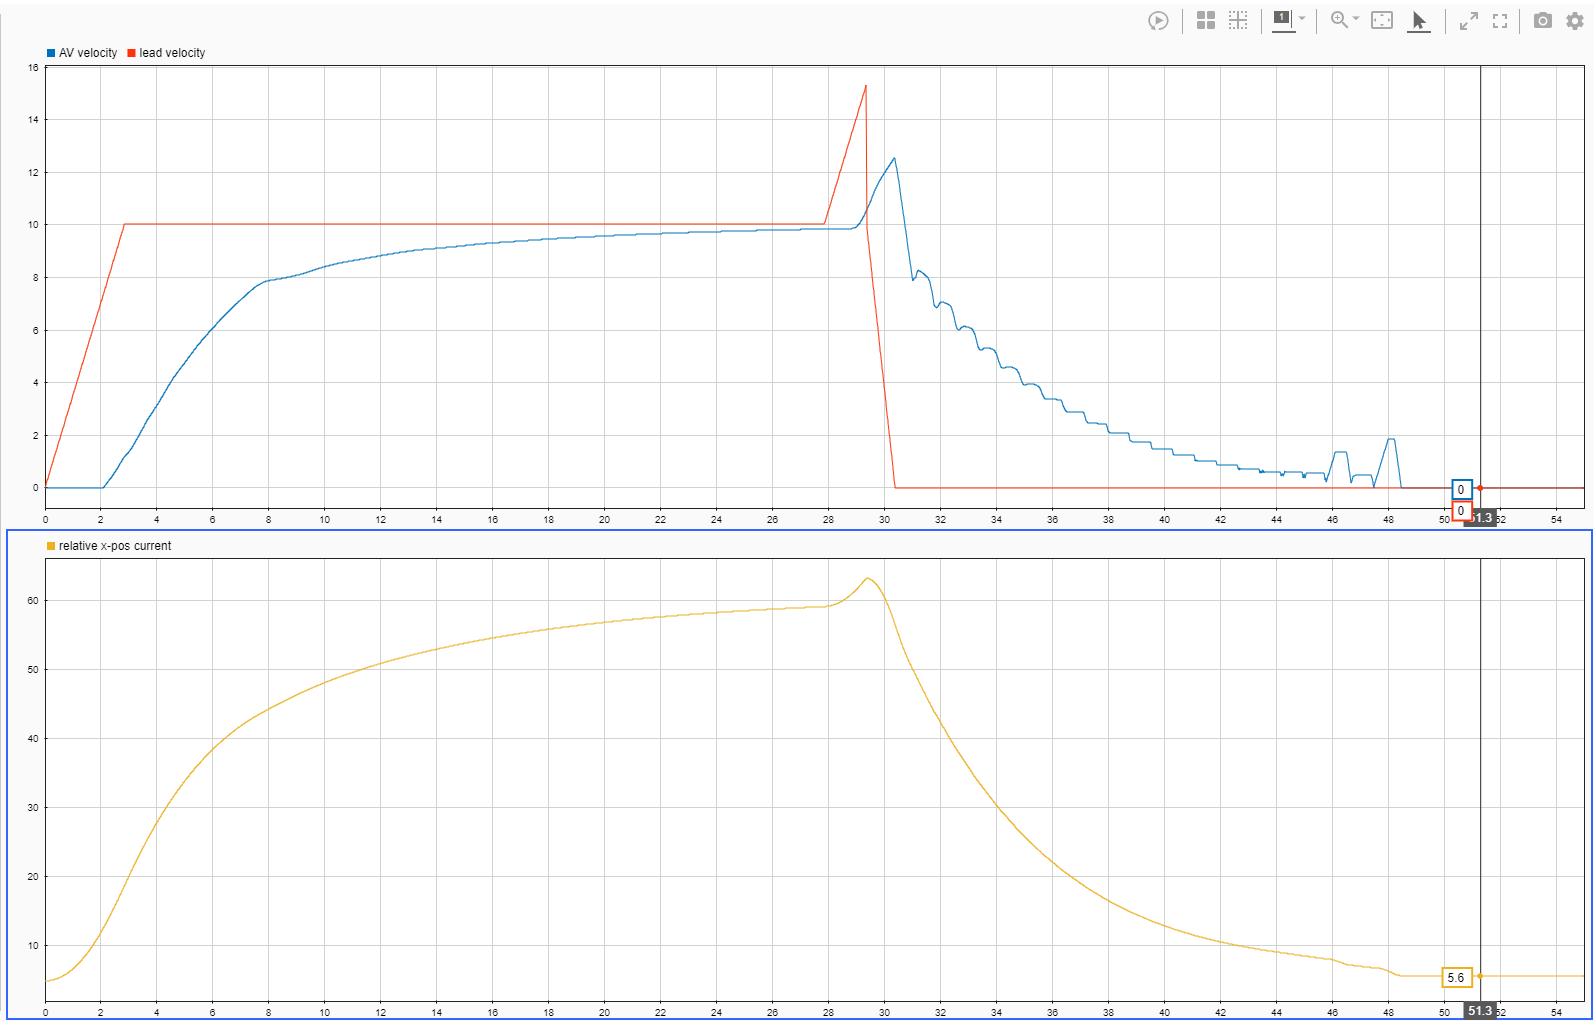
\includegraphics[width=5.71 in]{newFS_safety2.PNG}}
\caption{New FollowerStopper in Safety Test 2.}
\label{newsafe2}
\end{figure}

\begin{figure}[htbp]
\centerline{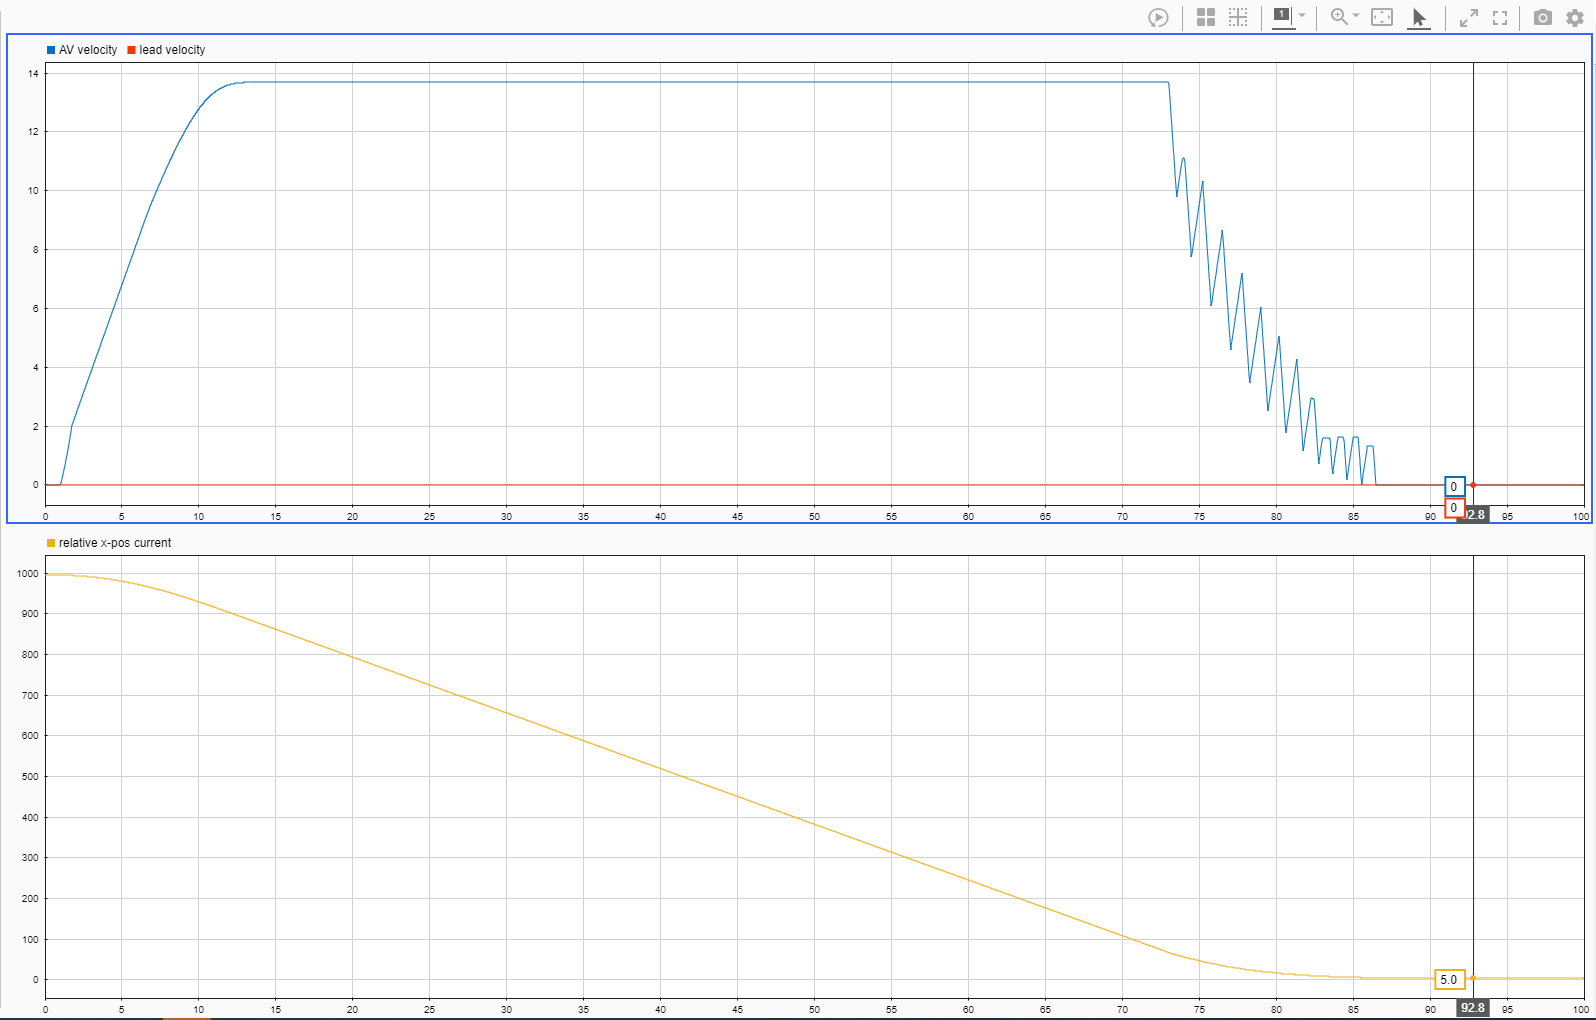
\includegraphics[width=5.71 in]{newFS_safety3.PNG}}
\caption{New FollowerStopper in Safety Test 3.}
\label{newsafe3}
\end{figure}


\pagebreak
\subsection{FollowerStopper string stability plots}

\begin{figure}[htbp]
\centerline{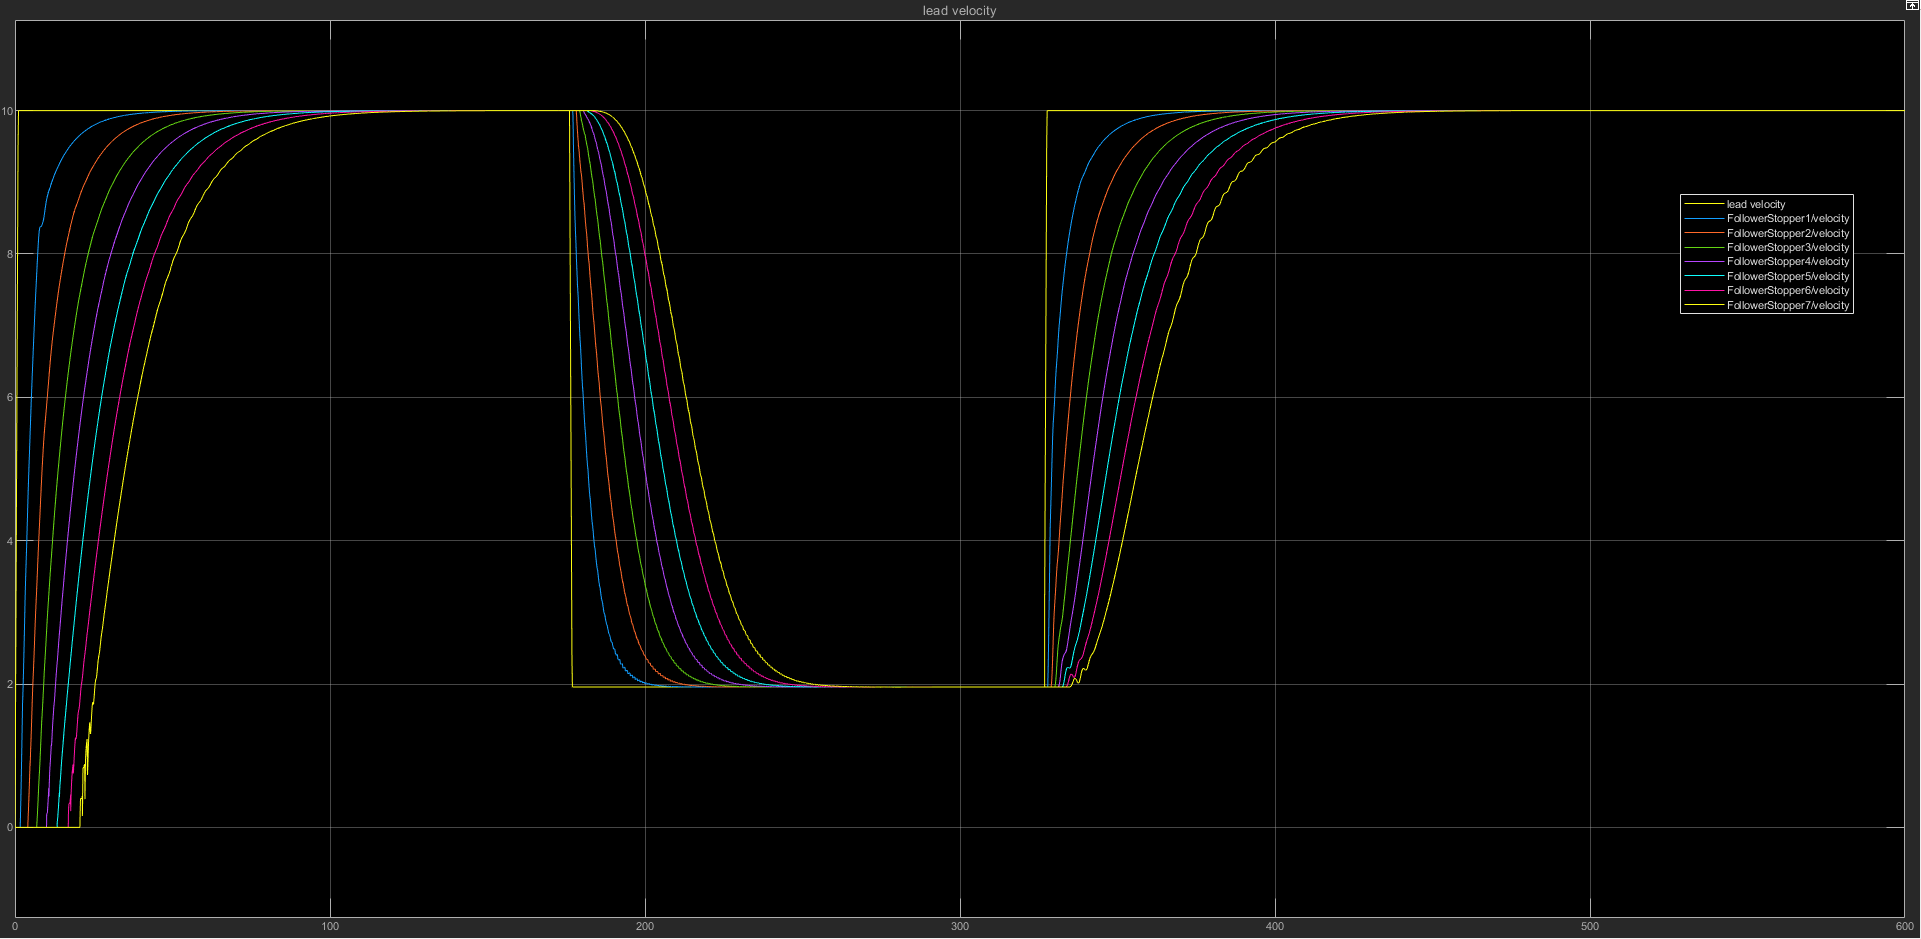
\includegraphics[width=6.50 in]{multiFS_velbad.PNG}}
\caption{Velocity vs time of seven-car FollowerStopper model in Step Test with bad reference velocity.}
\label{stringvelbad}
\end{figure}

\begin{figure}[htbp]
\centerline{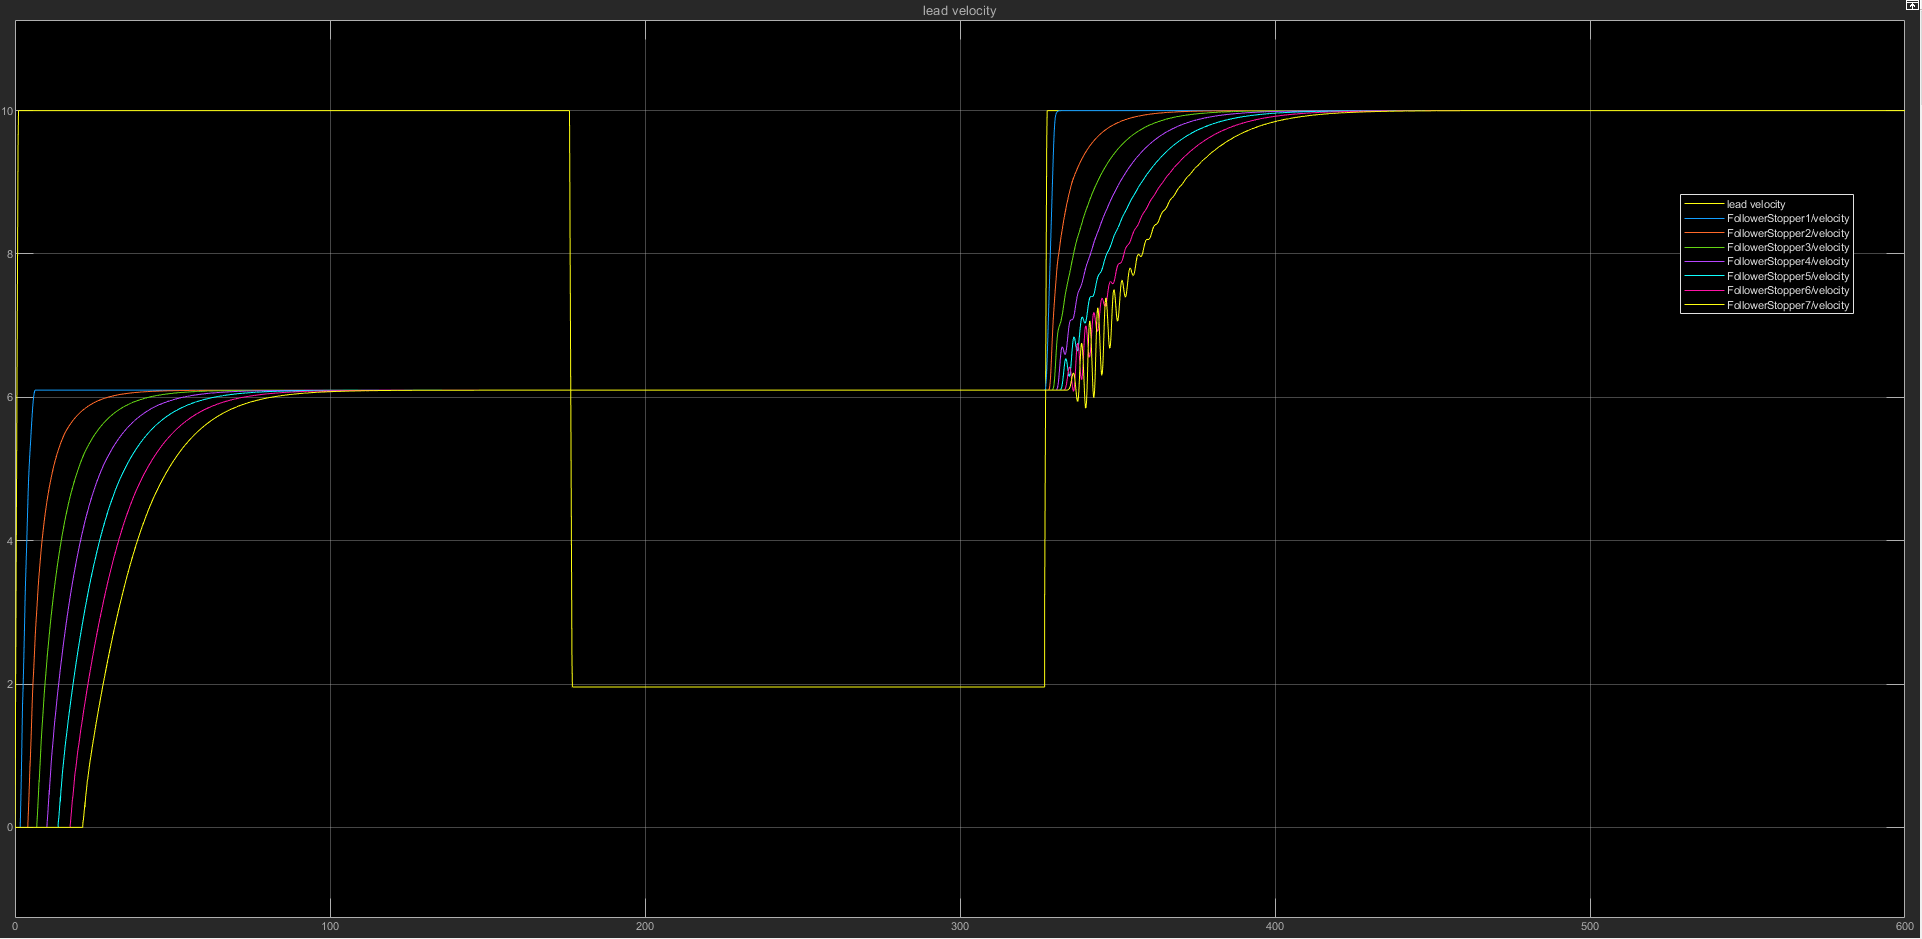
\includegraphics[width=6.50 in]{multiFS_velgood.PNG}}
\caption{Velocity vs time of seven-car FollowerStopper model in Step Test with good reference velocity.}
\label{stringvelgood}
\end{figure}

\begin{figure}[htbp]
\centerline{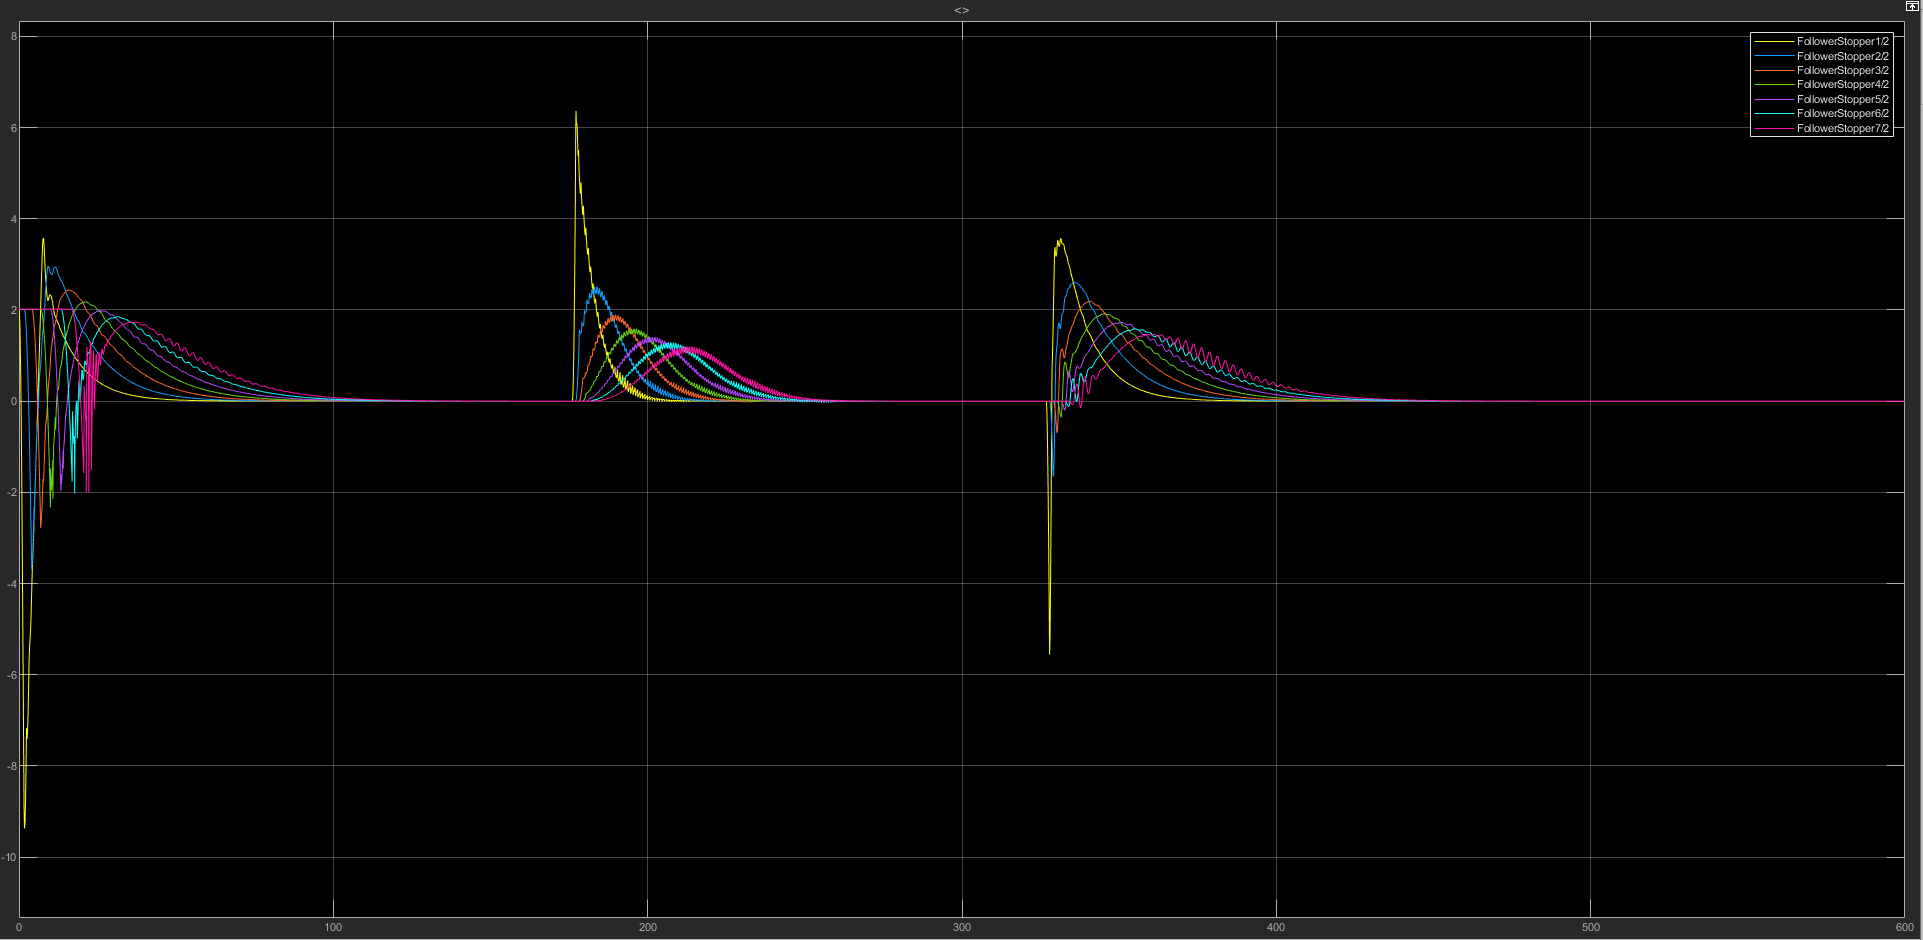
\includegraphics[width=6.50 in]{multiFS_errorbad.PNG}}
\caption{Spacing error vs time of seven-car FollowerStopper model in Step Test with bad reference velocity.}
\label{stringerrorbad}
\end{figure}

\begin{figure}[htbp]
\centerline{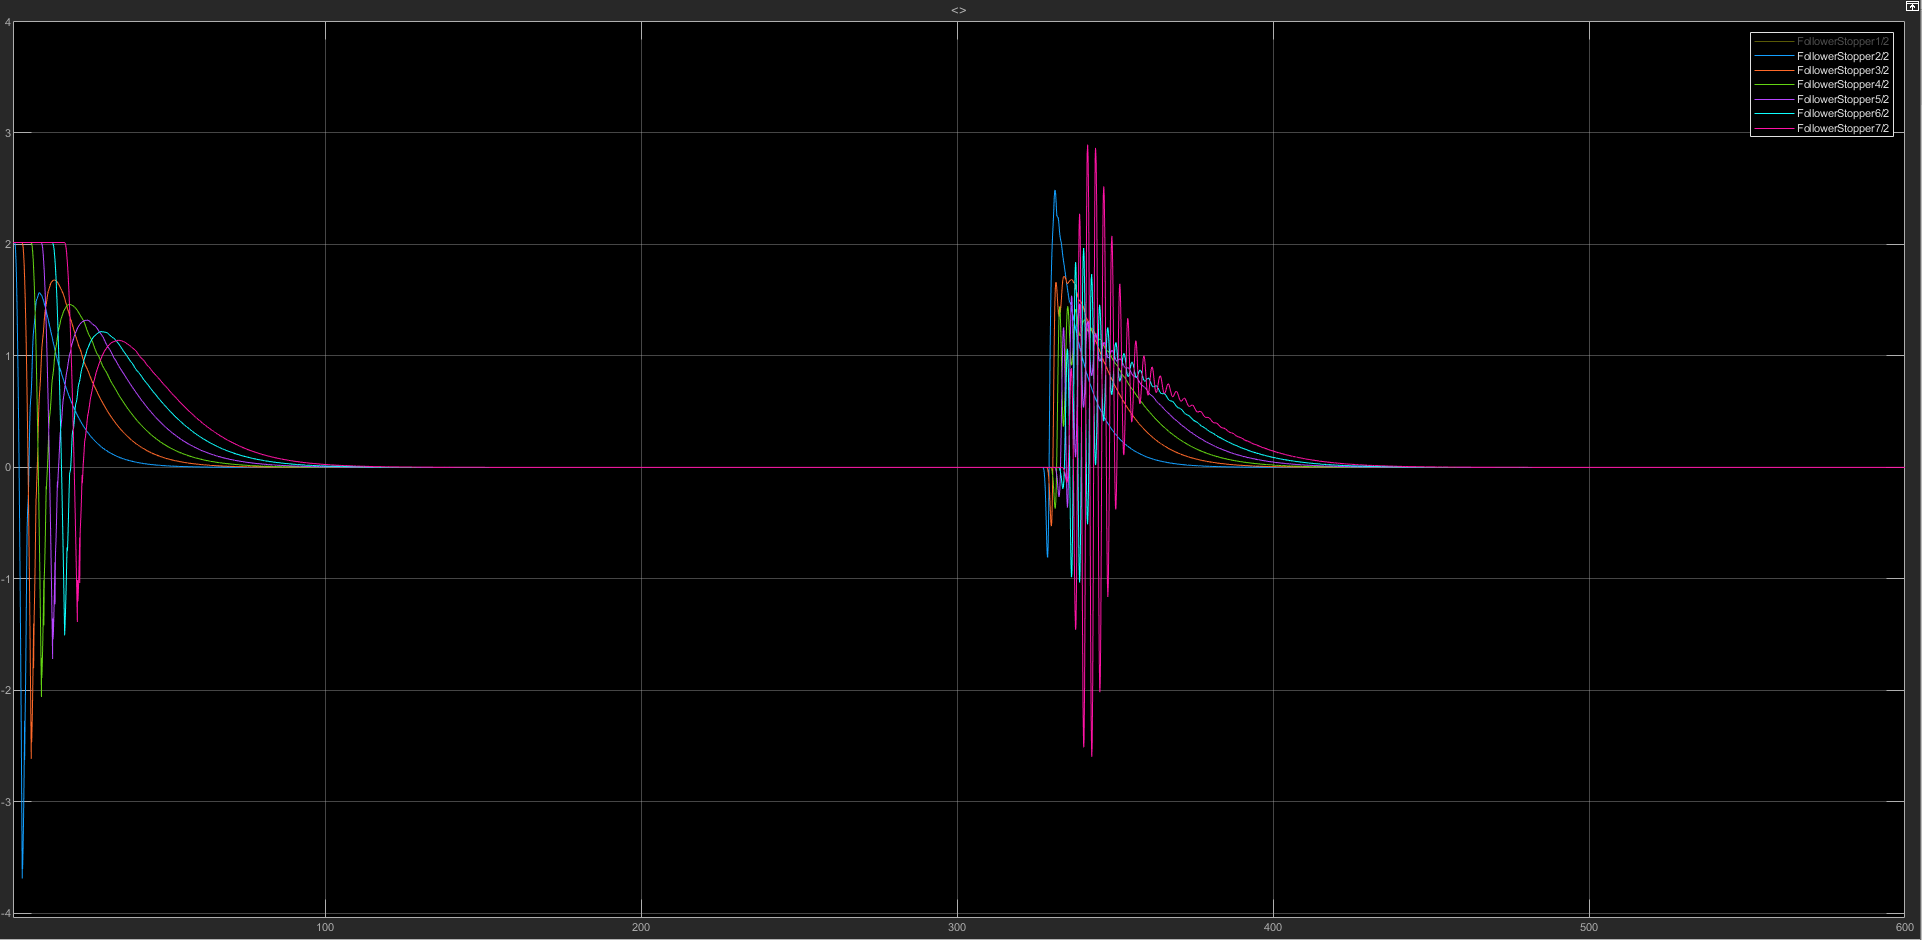
\includegraphics[width=6.50 in]{multiFS_errorgood.PNG}}
\caption{Spacing error vs time of seven-car FollowerStopper model in Step Test with good reference velocity.}
\label{stringerrorgood}
\end{figure}

\begin{figure}[htbp]
\centerline{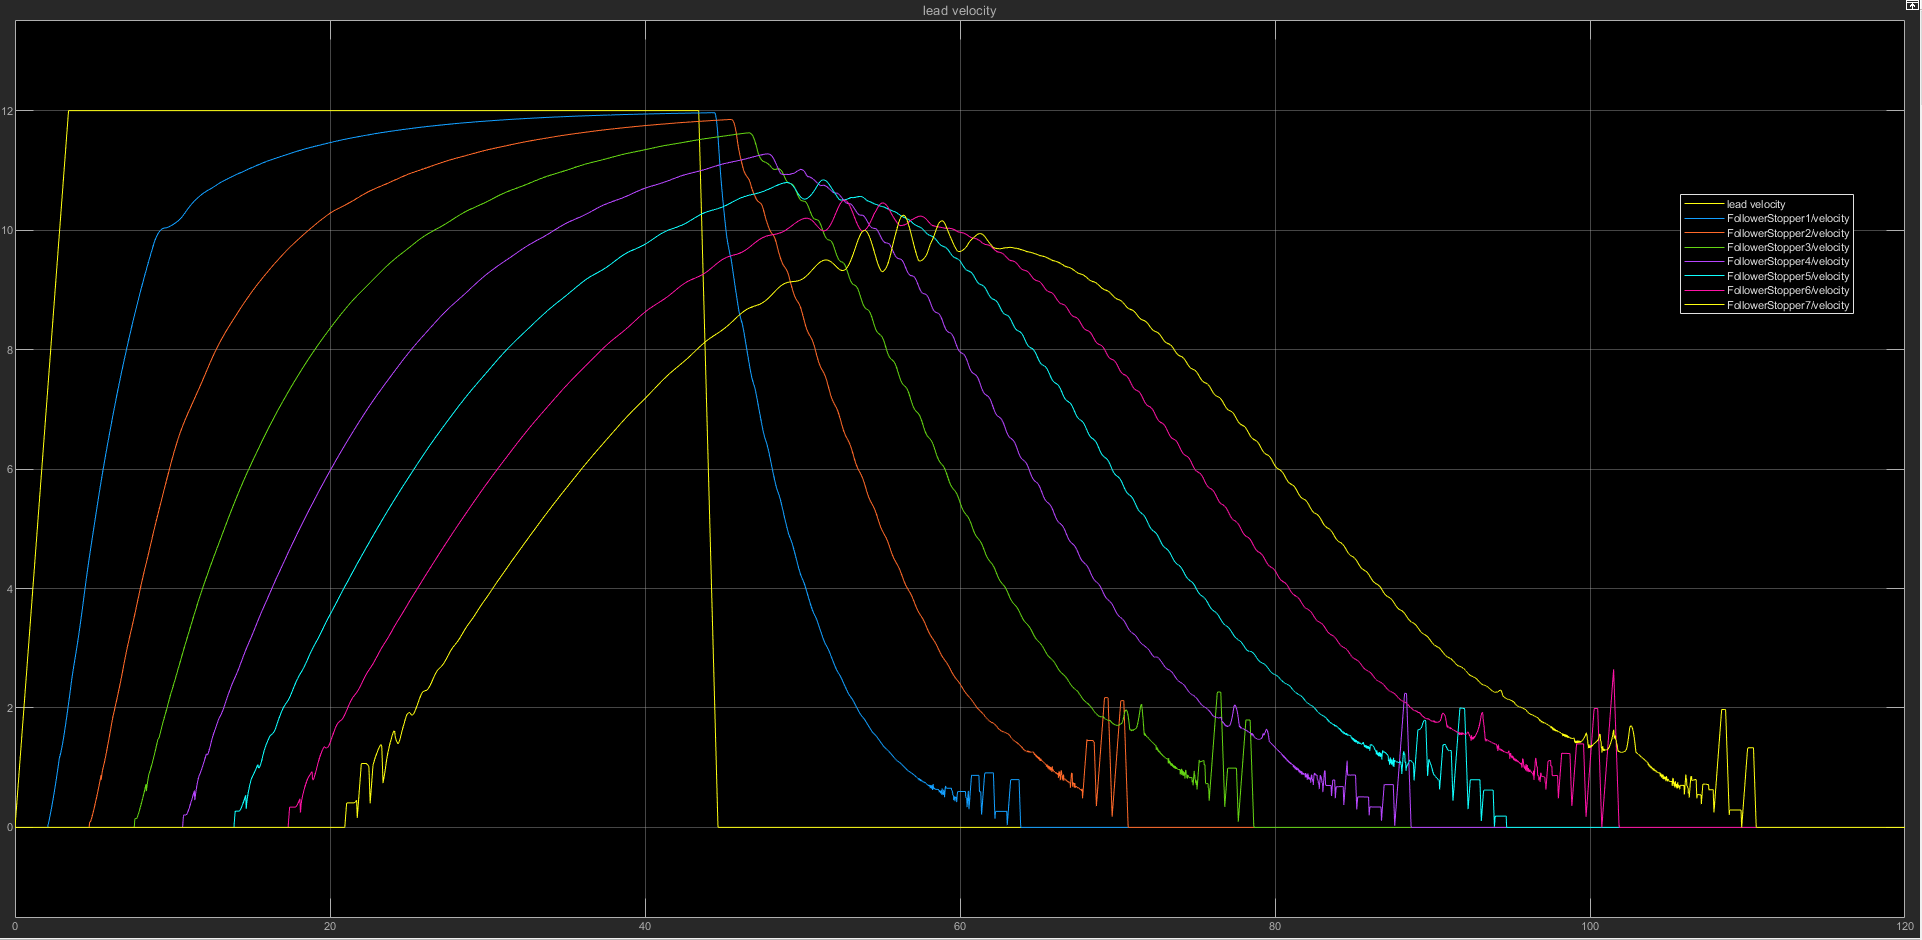
\includegraphics[width=6.50 in]{multiFS_safety1.PNG}}
\caption{Velocity vs time of seven-car FollowerStopper in Safety Test 1 with bad reference velocity.}
\label{stringsafety1}
\end{figure}

\end{appendix}
\end{document}
